
\section{Kết quả huấn luyện mô hình}

Trong phạm vi thực nghiệm hiện tại, dữ liệu huấn luyện được lấy từ 6 quỹ đạo artifact của kịch bản \texttt{chaos-pod-kill-product}. Các quỹ đạo này đã được ánh xạ về không gian trạng thái MDP và đưa vào môi trường \texttt{ArtifactReplayEnv} để huấn luyện tác nhân. Kết quả được lưu theo từng run, bao gồm mô hình, metadata và các biểu đồ chẩn đoán quá trình học.

\subsection{DQN}

Đối với DQN, mô hình được huấn luyện trong 400\,000 bước thời gian với môi trường động học \texttt{hybrid\_controlled}, hệ số nhiễu \texttt{noise\_scale = 0.70} và 40 episode đánh giá sau huấn luyện. Các siêu tham số chính của run này gồm \textit{learning rate} $= 5\times10^{-5}$, \textit{buffer size} = 200\,000, \textit{batch size} = 256, \textit{target update interval} = 2\,000 và cơ chế thăm dò \textit{epsilon-greedy} giảm từ 1.0 xuống 0.05.

\begin{minipage}{\textwidth}
    \centering
    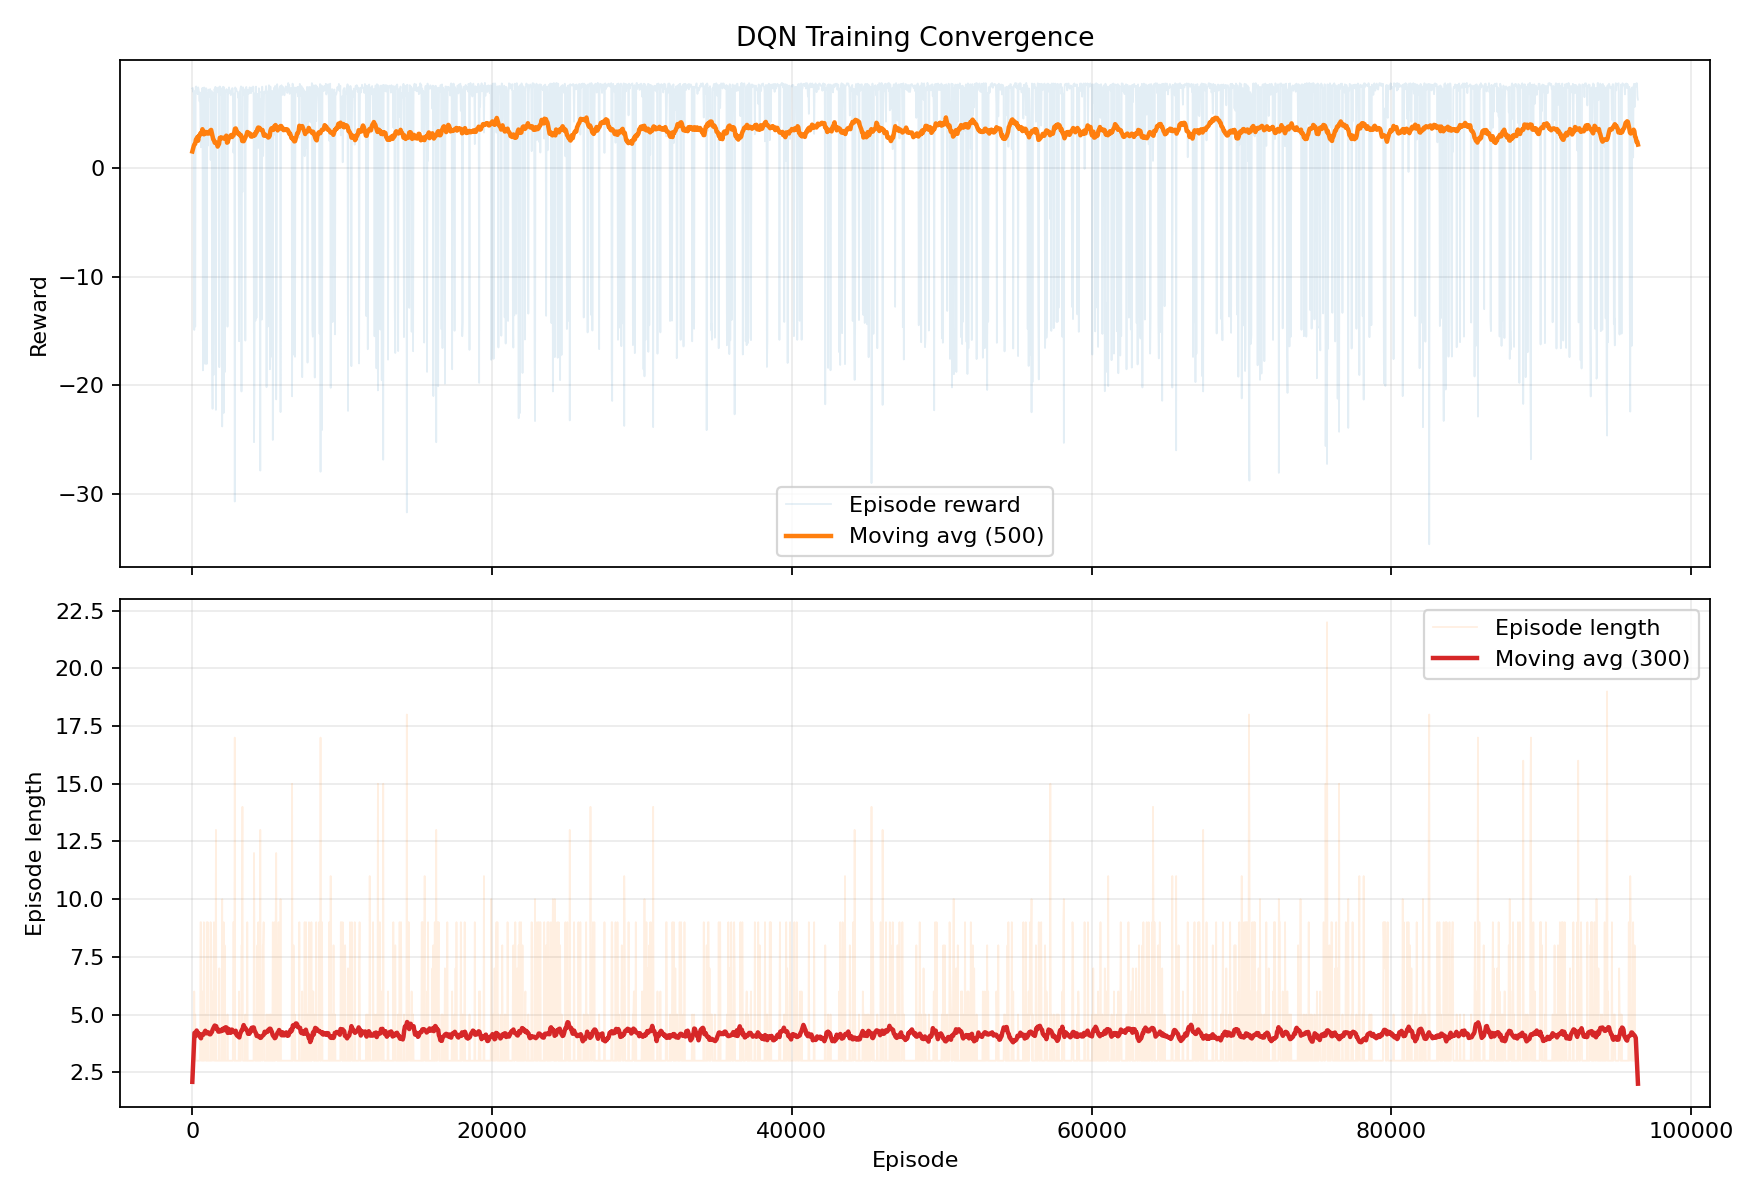
\includegraphics[width=0.95\textwidth]{graphics/chapter-6/train_DQN/training_curve.png}
    \captionsetup{hypcap=false}
    \captionof{figure}{Biểu đồ hội tụ theo phần thưởng và độ dài episode của DQN}
    \label{fig:dqn-training-convergence}
\end{minipage}

\noindent Hình \ref{fig:dqn-training-convergence} biểu diễn sự biến thiên của phần thưởng theo episode và độ dài episode của DQN trong quá trình huấn luyện. Đường màu xanh nhạt và màu cam nhạt biểu thị điểm thưởng tức thời và độ dài episode thực tế, trong khi các đường đậm nét thể hiện giá trị trung bình trượt tương ứng. Có thể thấy điểm thưởng trung bình tăng dần và tiệm cận mức ổn định quanh giá trị 3.0--4.0. Đồng thời, độ dài của episode nhanh chóng hội tụ về khoảng 4 bước hành động, cho thấy tác nhân đã tìm ra cách khôi phục hệ thống hiệu quả và rút ngắn thời gian xử lý sự cố.

\begin{minipage}{\textwidth}
    \centering
    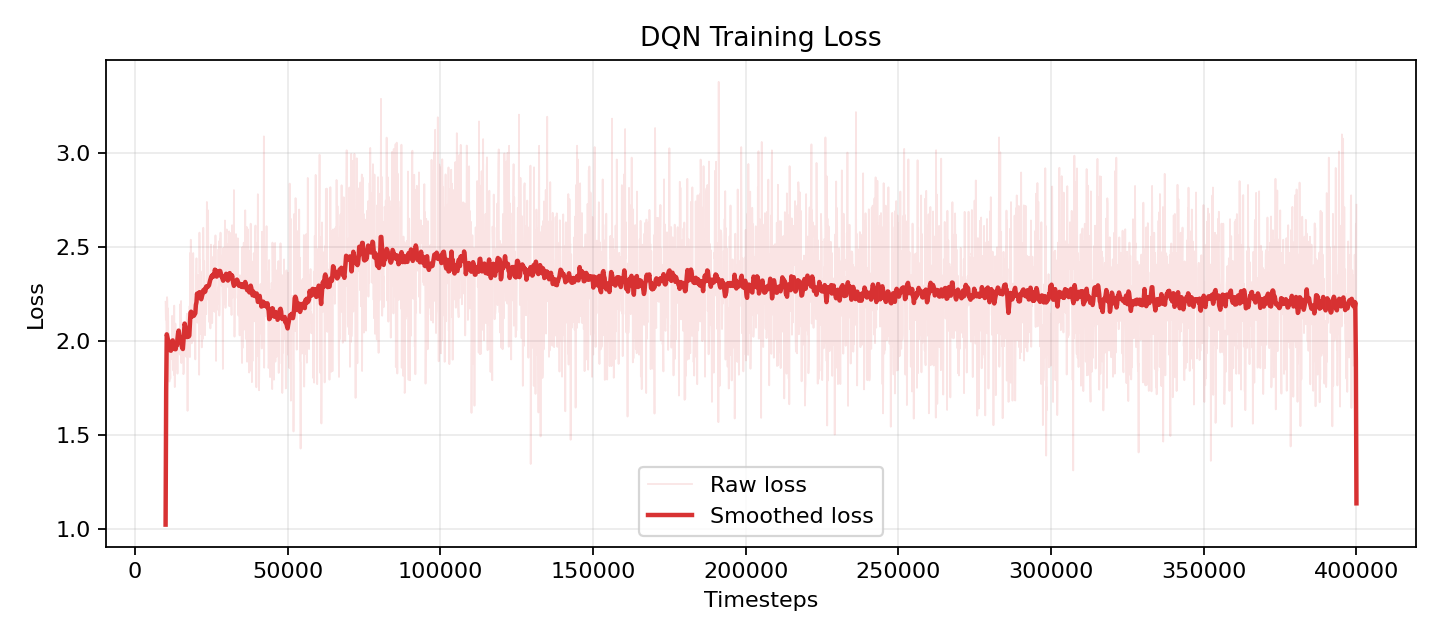
\includegraphics[width=0.9\textwidth]{graphics/chapter-6/train_DQN/loss_curve.png}
    \captionsetup{hypcap=false}
    \captionof{figure}{Biến thiên hàm mất mát (\textit{training loss}) của DQN}
    \label{fig:dqn-loss}
\end{minipage}

\noindent Đường biểu diễn hàm mất mát của mạng neural được trình bày ở Hình \ref{fig:dqn-loss}. Ở giai đoạn đầu, giá trị loss tăng vọt lên khoảng 2.5 do tác nhân bắt đầu khám phá và lưu trữ dữ liệu vào bộ nhớ đệm (\textit{replay buffer}), dẫn đến sai lệch lớn trong các bước cập nhật trọng số. Tuy nhiên, sau khoảng 80\,000 bước thời gian, hàm loss đi ngang và duy trì trạng thái ổn định quanh mức 2.2 cho tới cuối quá trình huấn luyện, đảm bảo mạng Q-learning không bị phân kỳ.

\begin{minipage}{\textwidth}
    \centering
    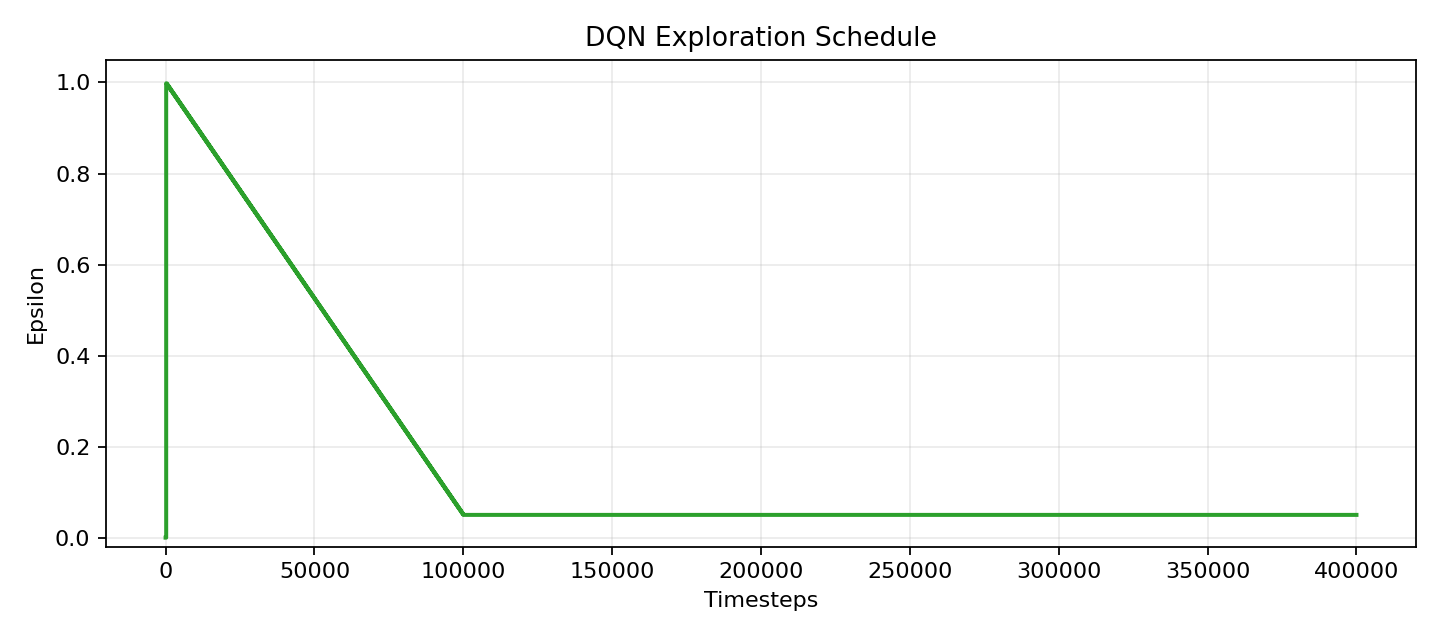
\includegraphics[width=0.9\textwidth]{graphics/chapter-6/train_DQN/epsilon_curve.png}
    \captionsetup{hypcap=false}
    \captionof{figure}{Lịch trình suy giảm hệ số thăm dò \textit{epsilon} của DQN}
    \label{fig:dqn-epsilon}
\end{minipage}

\noindent Lịch trình thăm dò của tác nhân DQN được mô tả ở Hình \ref{fig:dqn-epsilon}. Hệ số $\epsilon$ giảm tuyến tính từ 1.0 xuống 0.05 trong 100\,000 bước huấn luyện đầu tiên (chiếm 25\% tổng thời gian), sau đó giữ cố định ở mức 0.05. Lịch trình này đảm bảo tác nhân có đủ thời gian để khám phá các hành động ngẫu nhiên ở pha đầu trước khi chuyển hẳn sang khai thác chính sách tối ưu ở pha sau.

\begin{minipage}{\textwidth}
    \centering
    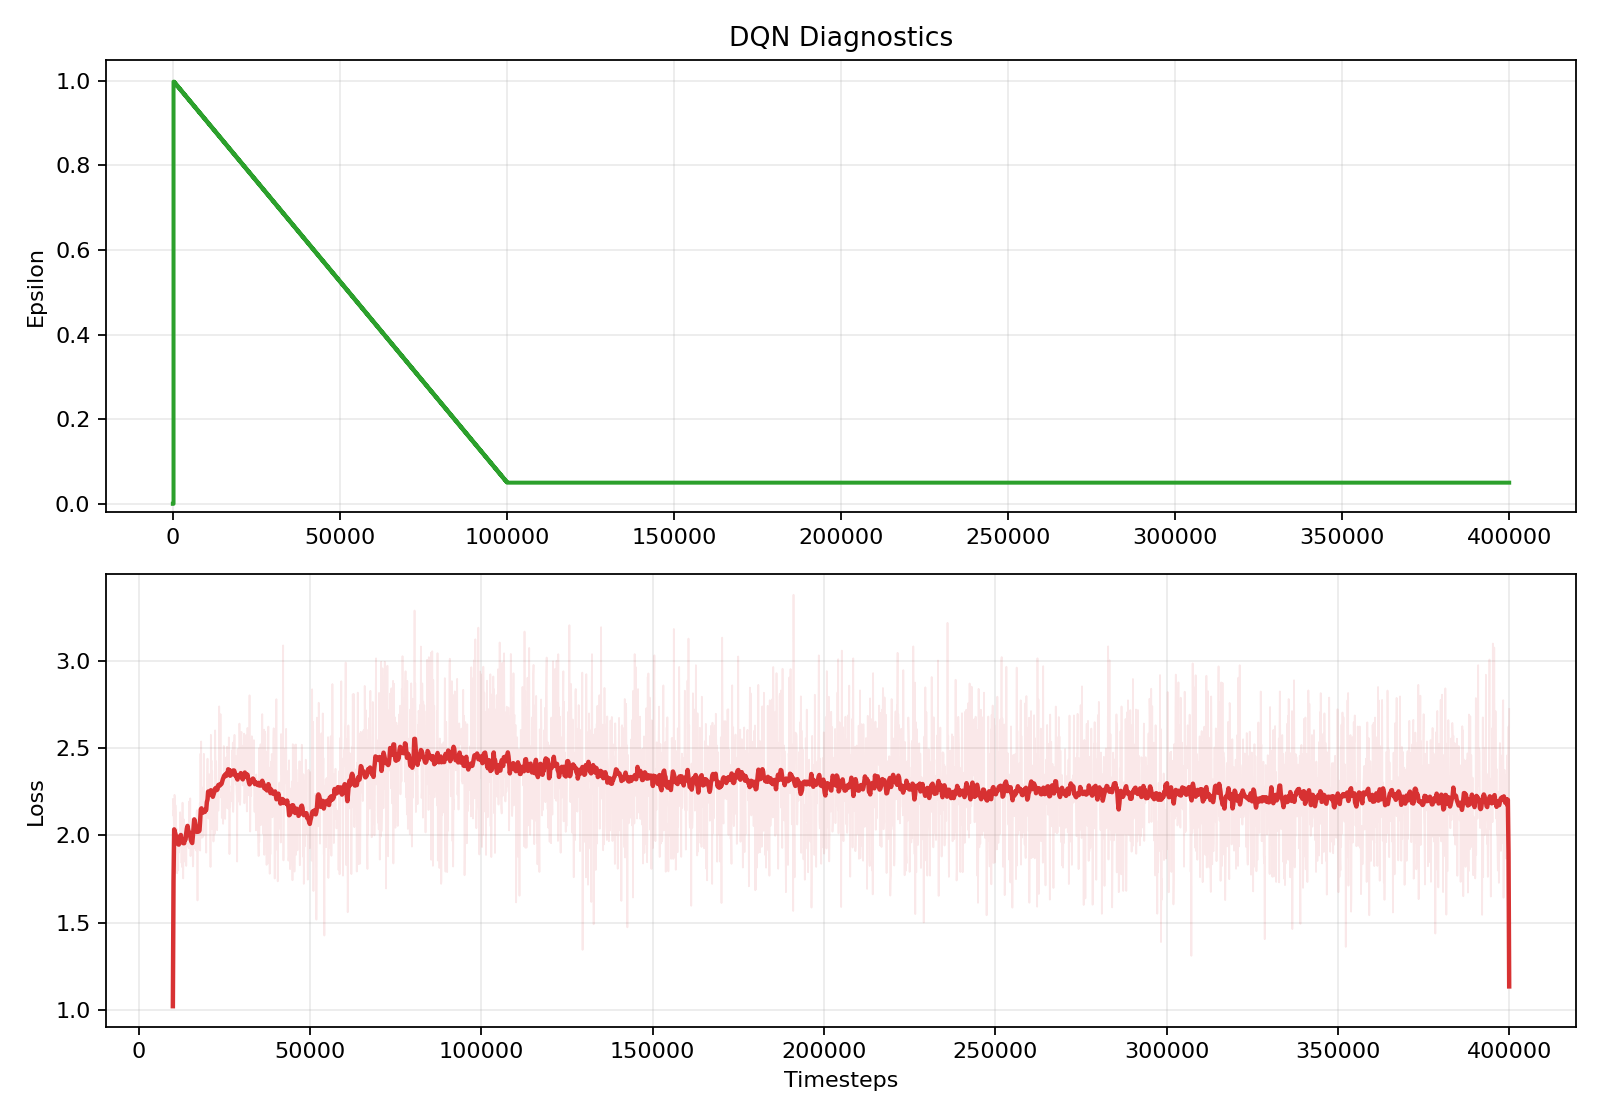
\includegraphics[width=0.92\textwidth]{graphics/chapter-6/train_DQN/dqn_diagnostics.png}
    \captionsetup{hypcap=false}
    \captionof{figure}{Biểu đồ chẩn đoán quá trình huấn luyện DQN tổng hợp}
    \label{fig:dqn-diagnostics-pod-failure}
\end{minipage}

\noindent Hình \ref{fig:dqn-diagnostics-pod-failure} tổng hợp hai chỉ số chẩn đoán quan trọng là hệ số $\epsilon$ và giá trị loss theo các bước thời gian. Sự kết hợp này giúp đối chiếu trực quan tiến trình huấn luyện, xác nhận rằng khi pha khám phá giảm dần, quá trình cập nhật giá trị Q cũng đi vào trạng thái ổn định và hội tụ.

\begin{minipage}{\textwidth}
    \centering
    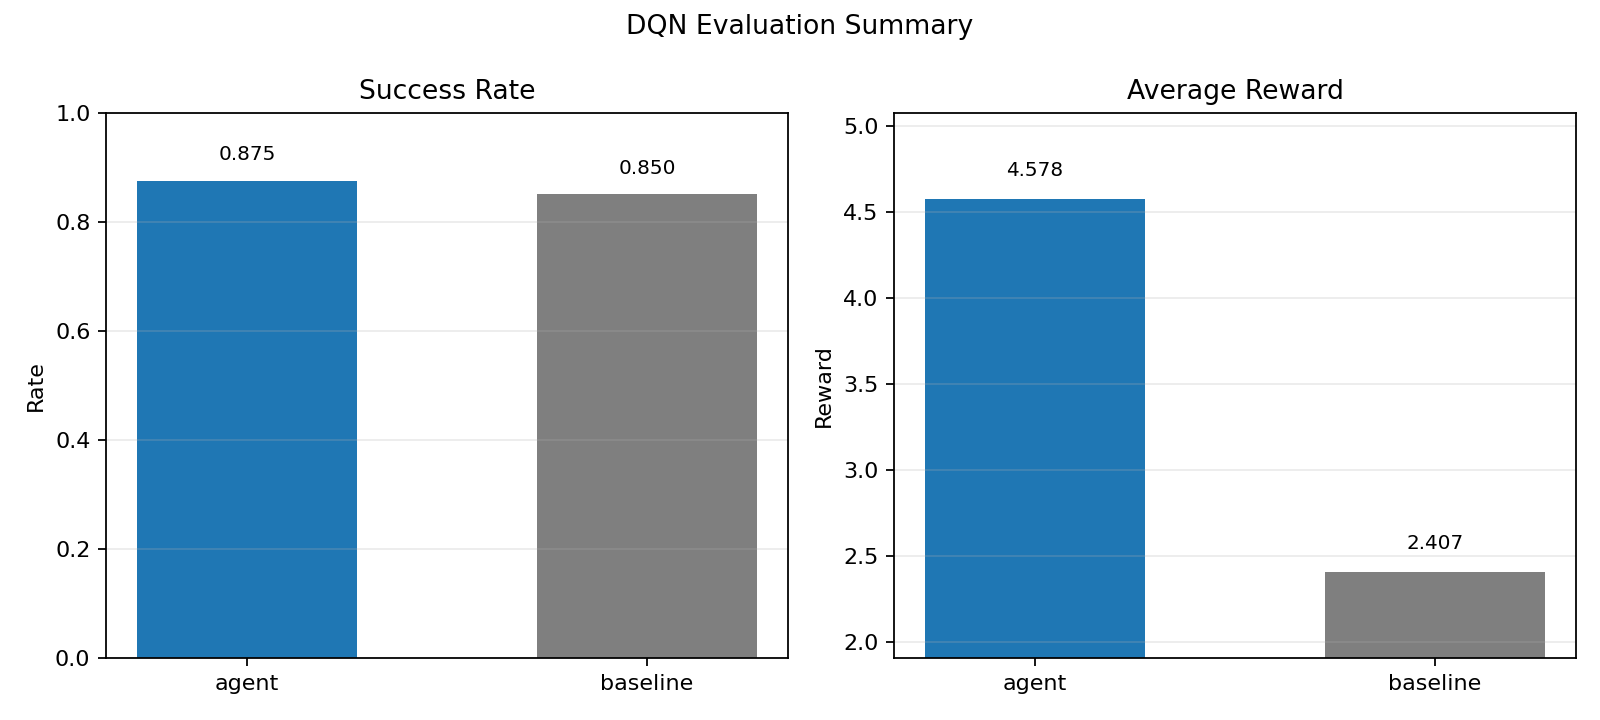
\includegraphics[width=0.92\textwidth]{graphics/chapter-6/train_DQN/evaluation_summary.png}
    \captionsetup{hypcap=false}
    \captionof{figure}{So sánh kết quả đánh giá DQN với baseline}
    \label{fig:dqn-evaluation-summary}
\end{minipage}

\noindent Kết quả đánh giá tác nhân DQN được trình bày ở Hình \ref{fig:dqn-evaluation-summary}. Sau khi hoàn thành huấn luyện, mô hình DQN đạt tỷ lệ phục hồi thành công (\textit{success rate}) là 0.875, cao hơn so với mức 0.850 của baseline ngẫu nhiên. Về mặt tối ưu hóa chi phí và hiệu năng hệ thống, phần thưởng trung bình của DQN đạt 4.578, vượt trội đáng kể so với baseline (2.407). Điều này chứng minh tác nhân đã học được cách giảm thiểu các hành động can thiệp thừa hoặc trùng lặp, nâng cao hiệu quả tự phục hồi cho hệ thống Kubernetes.

\subsection{A2C}

Đối với A2C, mô hình được huấn luyện trong 300\,000 bước thời gian với kịch bản động học \texttt{hybrid\_controlled}, hệ số nhiễu \texttt{noise\_scale = 0.65} và 40 episode đánh giá sau huấn luyện. Các siêu tham số cấu hình chính bao gồm tốc độ học \textit{learning rate} $= 10^{-4}$ (sử dụng lịch trình thay đổi tuyến tính), số bước cập nhật mỗi chu kỳ \textit{n\_steps} = 64, hệ số giảm giá \textit{gamma} = 0.995, tham số \textit{gae\_lambda} = 0.97, hệ số entropy \textit{ent\_coef} = 0.001 và hệ số hàm giá trị \textit{vf\_coef} = 0.5.

\begin{minipage}{\textwidth}
    \centering
    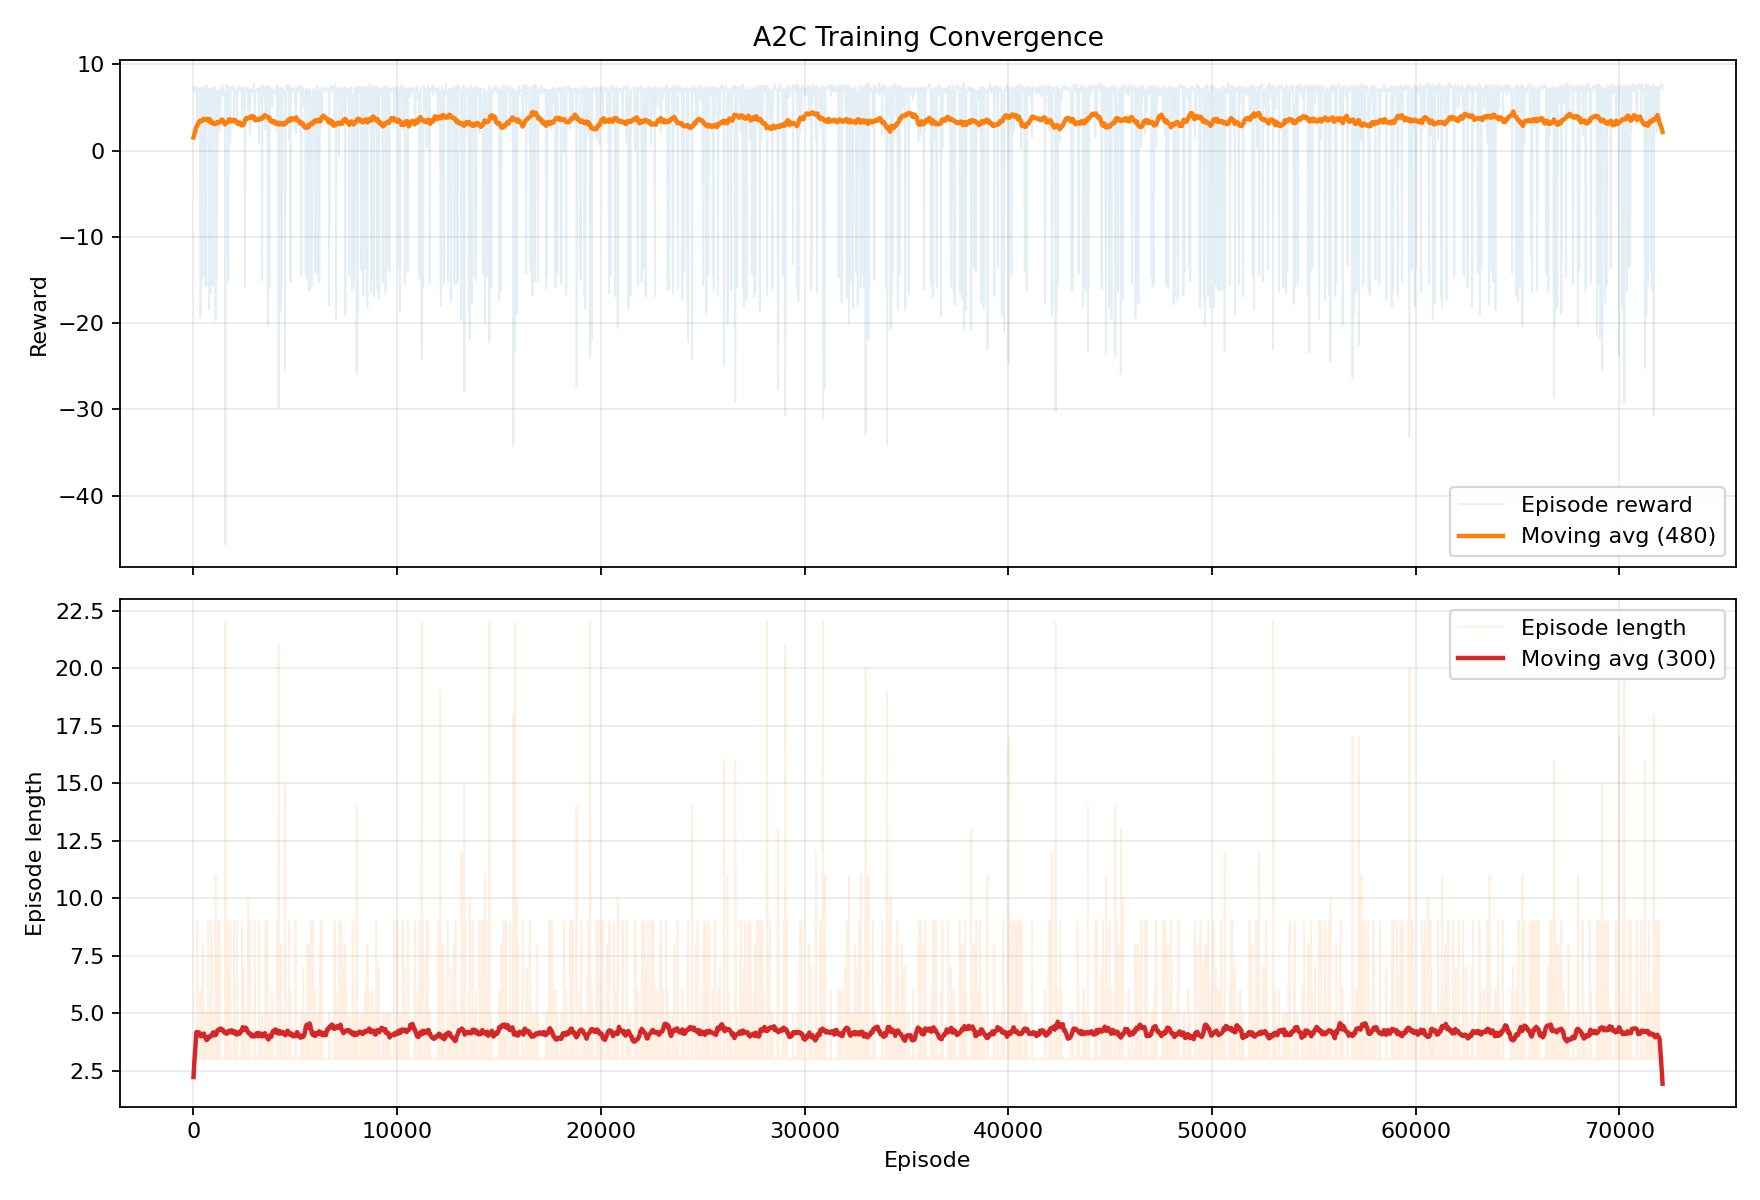
\includegraphics[width=0.95\textwidth]{graphics/chapter-6/train_A2C/training_curve.png}
    \captionsetup{hypcap=false}
    \captionof{figure}{Biểu đồ hội tụ theo phần thưởng và độ dài episode của A2C}
    \label{fig:a2c-training-convergence}
\end{minipage}

\noindent Hình \ref{fig:a2c-training-convergence} mô tả quá trình hội tụ phần thưởng và độ dài episode trong suốt 300\,000 bước huấn luyện của tác nhân A2C. Mặc dù điểm thưởng tức thời (đường màu xanh nhạt) vẫn dao động lớn do tính chất ngẫu nhiên của môi trường K8s giả lập, đường trung bình trượt (đường màu cam) cho thấy xu hướng tăng trưởng rõ nét từ mức 2.0 lên tiệm cận mức 6.5 và ổn định hoàn toàn ở nửa sau quá trình huấn luyện. Đồng thời, độ dài trung bình của mỗi episode (đường màu đỏ) duy trì ổn định quanh mức 4 bước can thiệp, chứng minh tác nhân đã nhanh chóng tìm được phương án phục hồi tối ưu.

\begin{minipage}{\textwidth}
    \centering
    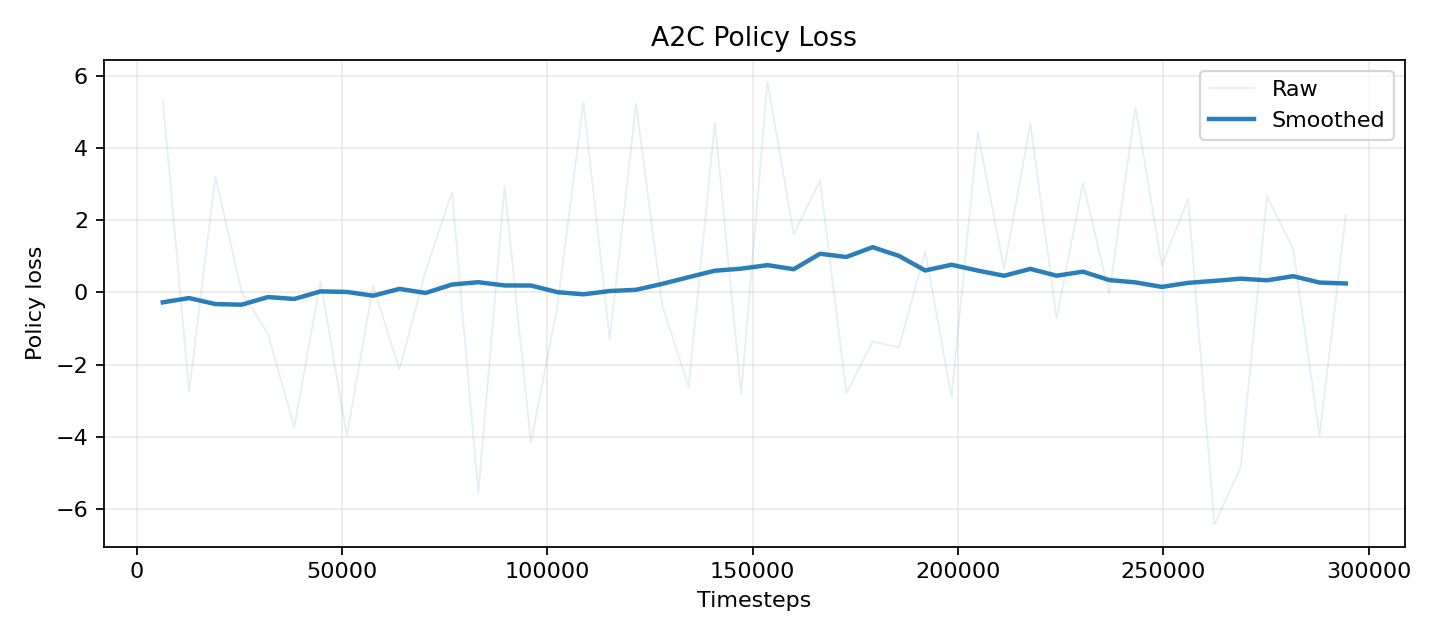
\includegraphics[width=0.9\textwidth]{graphics/chapter-6/train_A2C/policy_loss_curve.png}
    \captionsetup{hypcap=false}
    \captionof{figure}{Biến thiên \textit{policy loss} trong quá trình huấn luyện A2C}
    \label{fig:a2c-policy-loss}
\end{minipage}

\noindent Biến thiên hàm mất mát chính sách (\textit{policy loss}) của A2C được thể hiện trong Hình \ref{fig:a2c-policy-loss}. Do A2C cập nhật chính sách dựa trên hàm lợi thế (\textit{advantage function}), giá trị \textit{policy loss} dao động mạnh quanh điểm cân bằng 0 (trong khoảng [-6, 6]). Tuy nhiên, đường làm mượt (smoothed) cho thấy xu hướng ổn định tiệm cận về sát 0 ở các bước huấn luyện cuối cùng, khẳng định chính sách đã đi vào trạng thái hội tụ cục bộ.

\begin{minipage}{\textwidth}
    \centering
    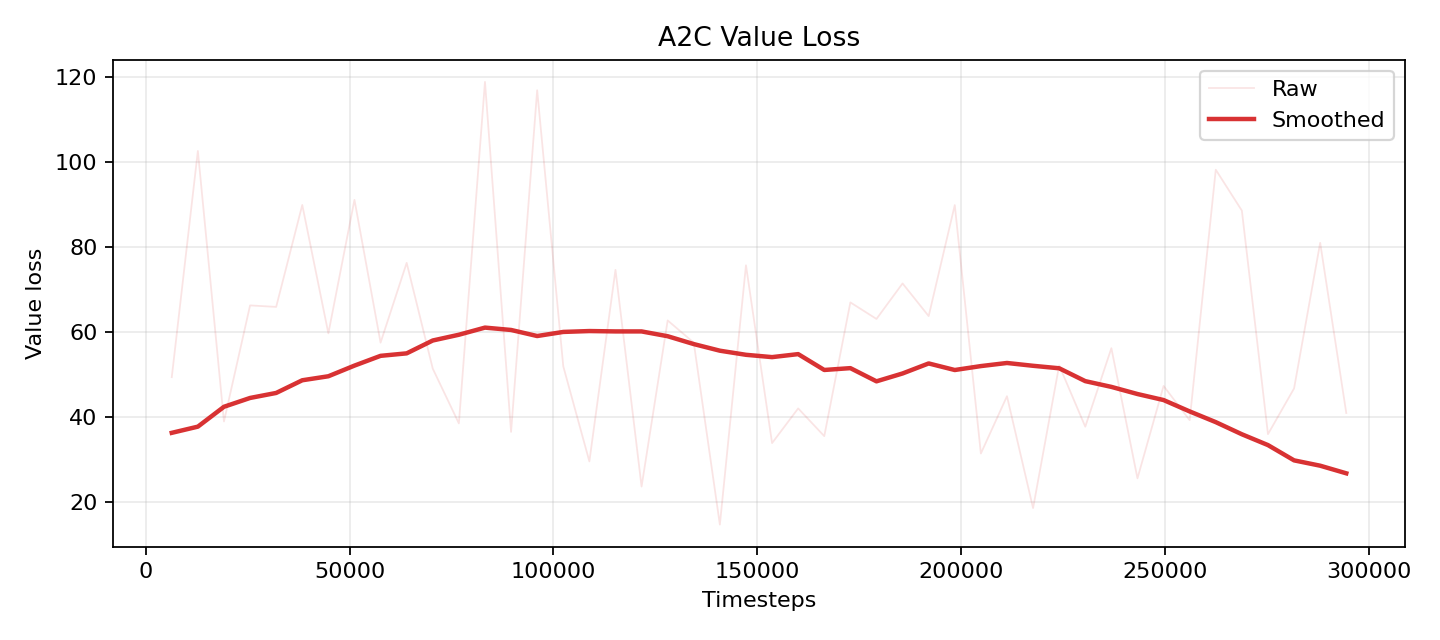
\includegraphics[width=0.9\textwidth]{graphics/chapter-6/train_A2C/value_loss_curve.png}
    \captionsetup{hypcap=false}
    \captionof{figure}{Biến thiên \textit{value loss} của A2C}
    \label{fig:a2c-value-loss}
\end{minipage}

\noindent Hình \ref{fig:a2c-value-loss} biểu diễn biến thiên của hàm mất mát giá trị (\textit{value loss}) phản ánh sai số dự báo phần thưởng tích lũy của Critic. Hàm mất mát này ban đầu tăng từ 36 lên đỉnh điểm quanh mức 60 tại 100\,000 bước do tác nhân liên tục khám phá các trạng thái mới chưa có trong bộ nhớ. Sau khi mạng Critic học được xấp xỉ giá trị trạng thái tốt hơn, \textit{value loss} giảm dần về mức dưới 30 ở cuối quá trình huấn luyện, cho thấy chất lượng đánh giá trạng thái ngày càng chính xác.

\begin{minipage}{\textwidth}
    \centering
    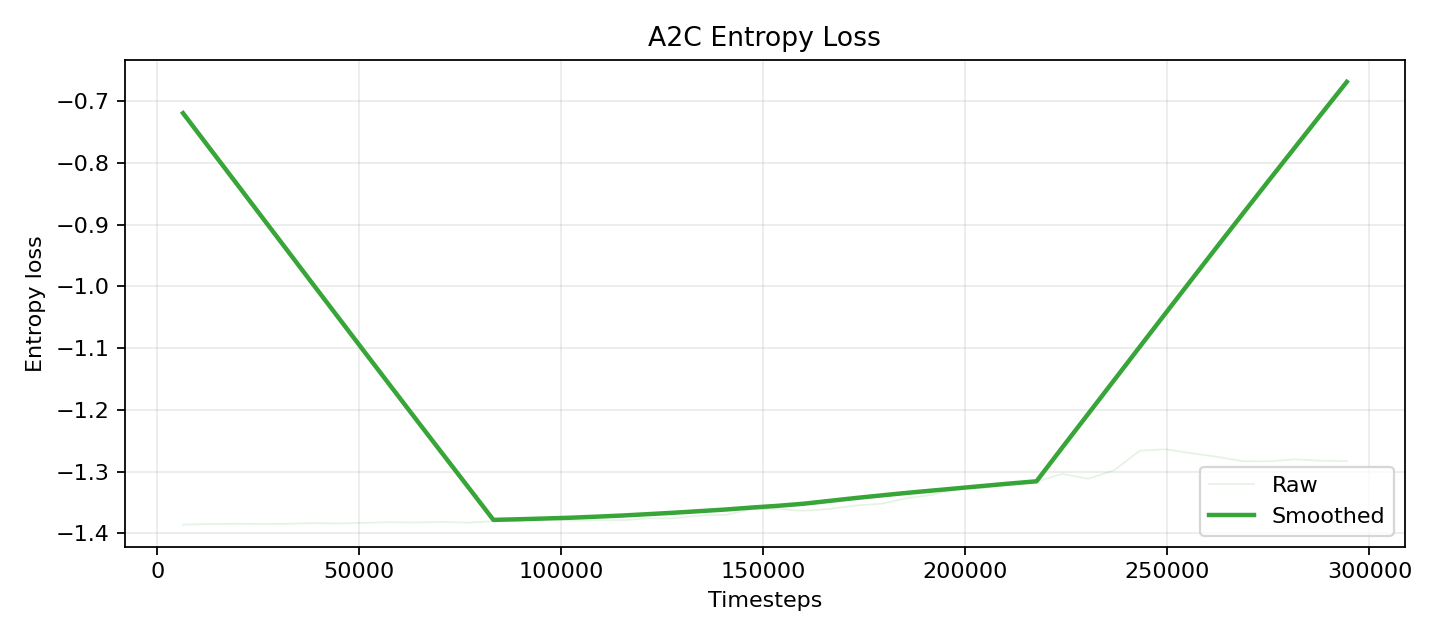
\includegraphics[width=0.9\textwidth]{graphics/chapter-6/train_A2C/entropy_curve.png}
    \captionsetup{hypcap=false}
    \captionof{figure}{Biến thiên \textit{entropy loss} của A2C}
    \label{fig:a2c-entropy-loss}
\end{minipage}

\noindent Ở Hình \ref{fig:a2c-entropy-loss}, tổn thất entropy (\textit{entropy loss}) bắt đầu từ mức -0.72 và giảm mạnh xuống -1.38 trong 80\,000 bước đầu, cho thấy chính sách đang dần tập trung vào các hành động có độ tin cậy cao. Sau 220\,000 bước, entropy loss lại có xu hướng tăng trở lại lên mức -0.67, điều này phản ánh việc điều chỉnh chính sách hoặc ảnh hưởng từ tốc độ học (learning rate) giúp tác nhân tăng cường thăm dò trở lại để tránh hội tụ vào các cực trị địa phương kém tối ưu.

\begin{minipage}{\textwidth}
    \centering
    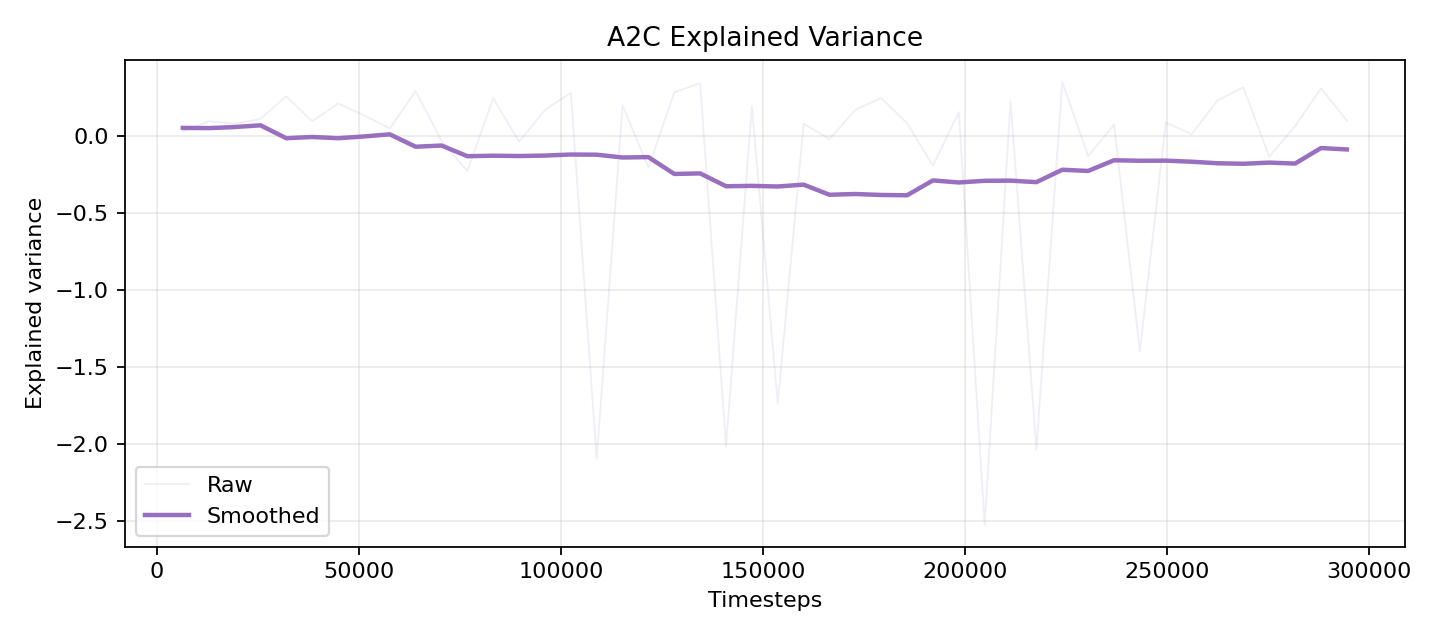
\includegraphics[width=0.92\textwidth]{graphics/chapter-6/train_A2C/explained_variance_curve.png}
    \captionsetup{hypcap=false}
    \captionof{figure}{Biến thiên sai số giải thích (\textit{explained variance}) của A2C}
    \label{fig:a2c-explained-variance}
\end{minipage}

\noindent Chỉ số phương sai giải thích (\textit{explained variance}) được biểu diễn trong Hình \ref{fig:a2c-explained-variance}. Chỉ số này đo lường mức độ dự báo chính xác của Critic đối với sự biến thiên phần thưởng. Giá trị \textit{explained variance} dao động chủ yếu trong khoảng từ 0.0 đến -0.4, phản ánh đặc trưng khó khăn trong việc dự đoán chính xác giá trị trạng thái trên môi trường có nhiễu động cao của hệ thống microservices.

\begin{minipage}{\textwidth}
    \centering
    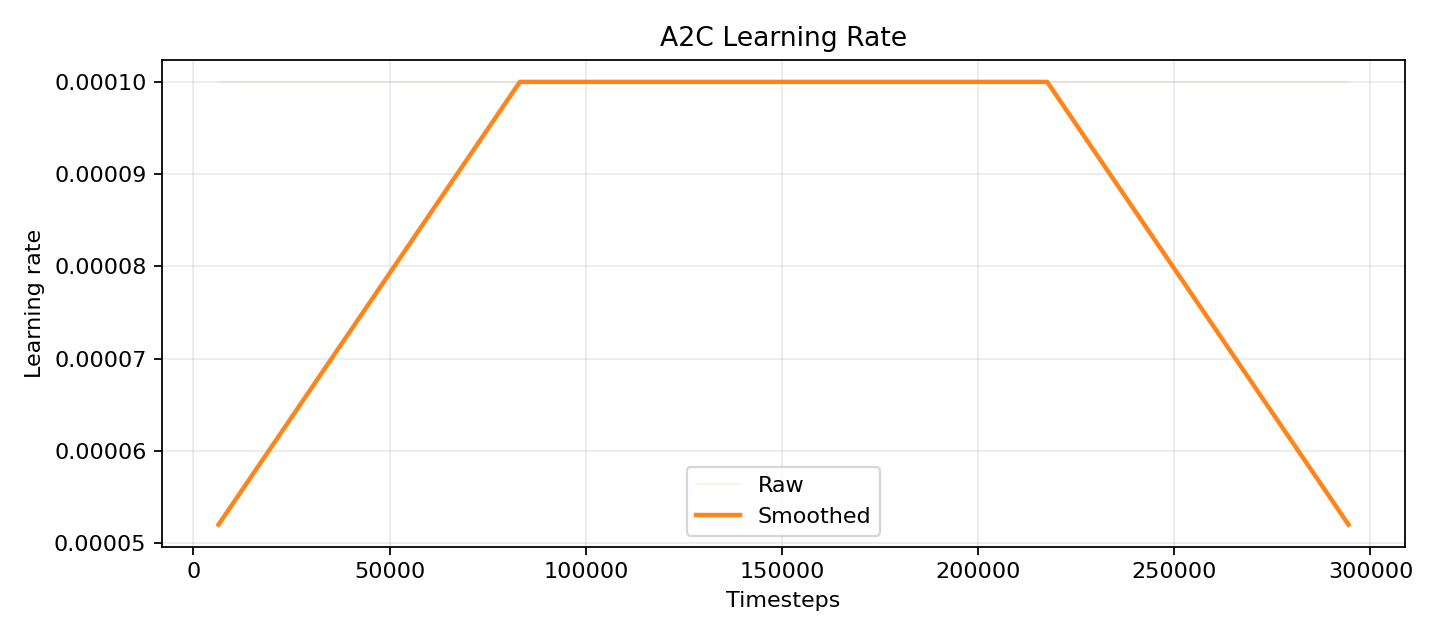
\includegraphics[width=0.9\textwidth]{graphics/chapter-6/train_A2C/learning_rate_curve.png}
    \captionsetup{hypcap=false}
    \captionof{figure}{Biến thiên tốc độ học trong quá trình huấn luyện A2C}
    \label{fig:a2c-learning-rate}
\end{minipage}

\noindent Hình \ref{fig:a2c-learning-rate} mô tả lịch trình thay đổi tốc độ học (\textit{learning rate}) của A2C. Tốc độ học được thiết lập tăng dần từ $5\times10^{-5}$ lên $10^{-4}$ trong 80\,000 bước đầu tiên để khởi động quá trình tối ưu hóa (warmup), duy trì ổn định đến bước thứ 220\,000, sau đó giảm dần về mức ban đầu ở bước thứ 300\,000 (cooldown). Lịch trình này giúp mô hình ổn định các bước đi gradient ở cả hai giai đoạn đầu và cuối huấn luyện.

\begin{minipage}{\textwidth}
    \centering
    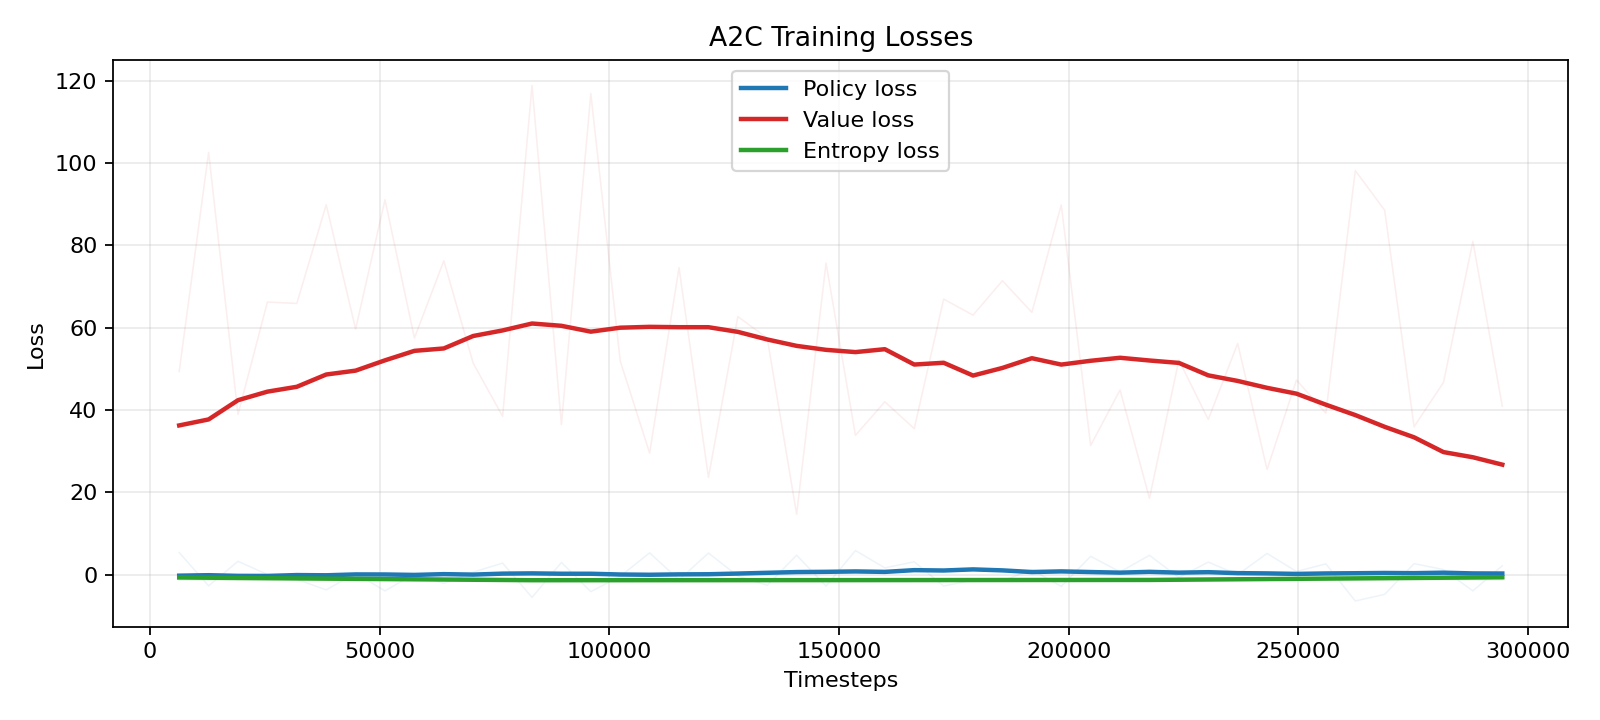
\includegraphics[width=0.92\textwidth]{graphics/chapter-6/train_A2C/loss_curve.png}
    \captionsetup{hypcap=false}
    \captionof{figure}{Biểu đồ tổng hợp các hàm mất mát chính của A2C}
    \label{fig:a2c-loss-summary}
\end{minipage}

\noindent Hình \ref{fig:a2c-loss-summary} tổng hợp đồng thời cả ba thành phần loss chính của thuật toán A2C. Biểu đồ cho thấy \textit{value loss} chiếm tỷ trọng lớn nhất về mặt thang đo, trong khi \textit{policy loss} và \textit{entropy loss} duy trì mức dao động nhỏ và ổn định xung quanh 0, đảm bảo tiến trình học song song của Actor và Critic diễn ra cân bằng.

\begin{minipage}{\textwidth}
    \centering
    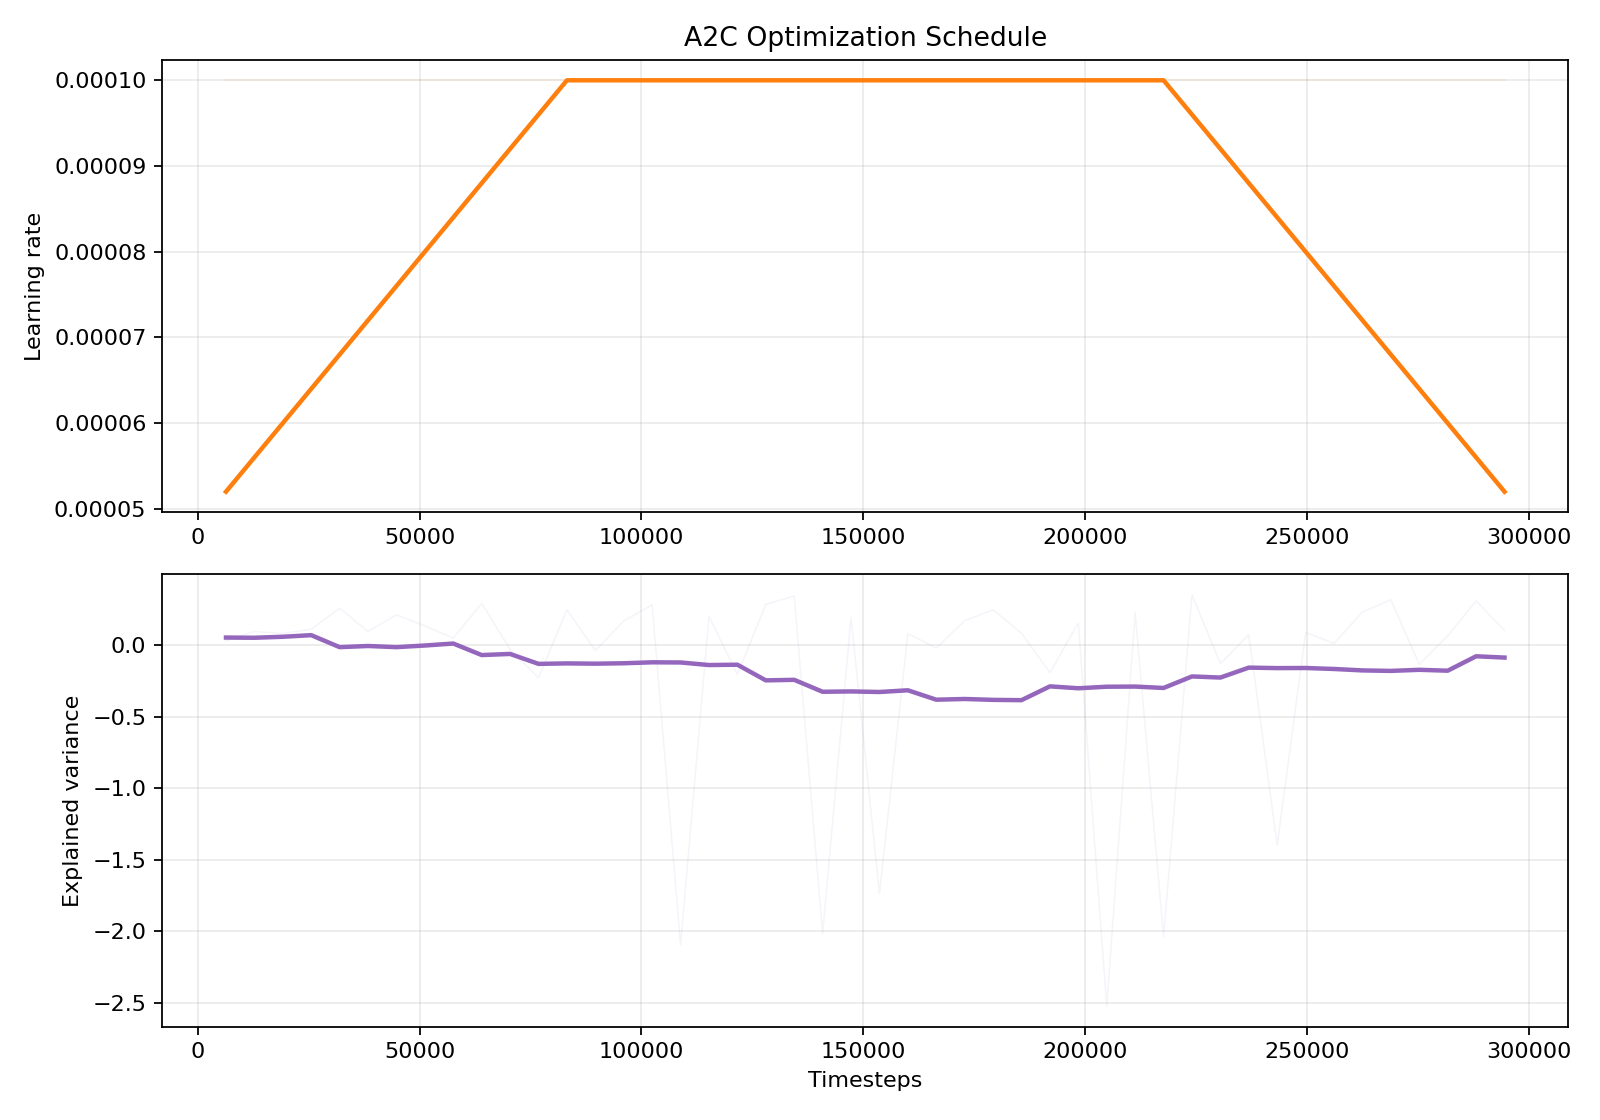
\includegraphics[width=0.92\textwidth]{graphics/chapter-6/train_A2C/optimization_curve.png}
    \captionsetup{hypcap=false}
    \captionof{figure}{Biểu đồ tổng hợp lịch tối ưu hóa của A2C}
    \label{fig:a2c-optimization-summary}
\end{minipage}

\noindent Hình \ref{fig:a2c-optimization-summary} tổng hợp lịch trình tốc độ học và sai số giải thích của A2C. Sự đối chiếu này cho thấy mối tương quan rõ rệt giữa việc thay đổi tốc độ học và tính ổn định của các chỉ số chẩn đoán tối ưu hóa.

\begin{minipage}{\textwidth}
    \centering
    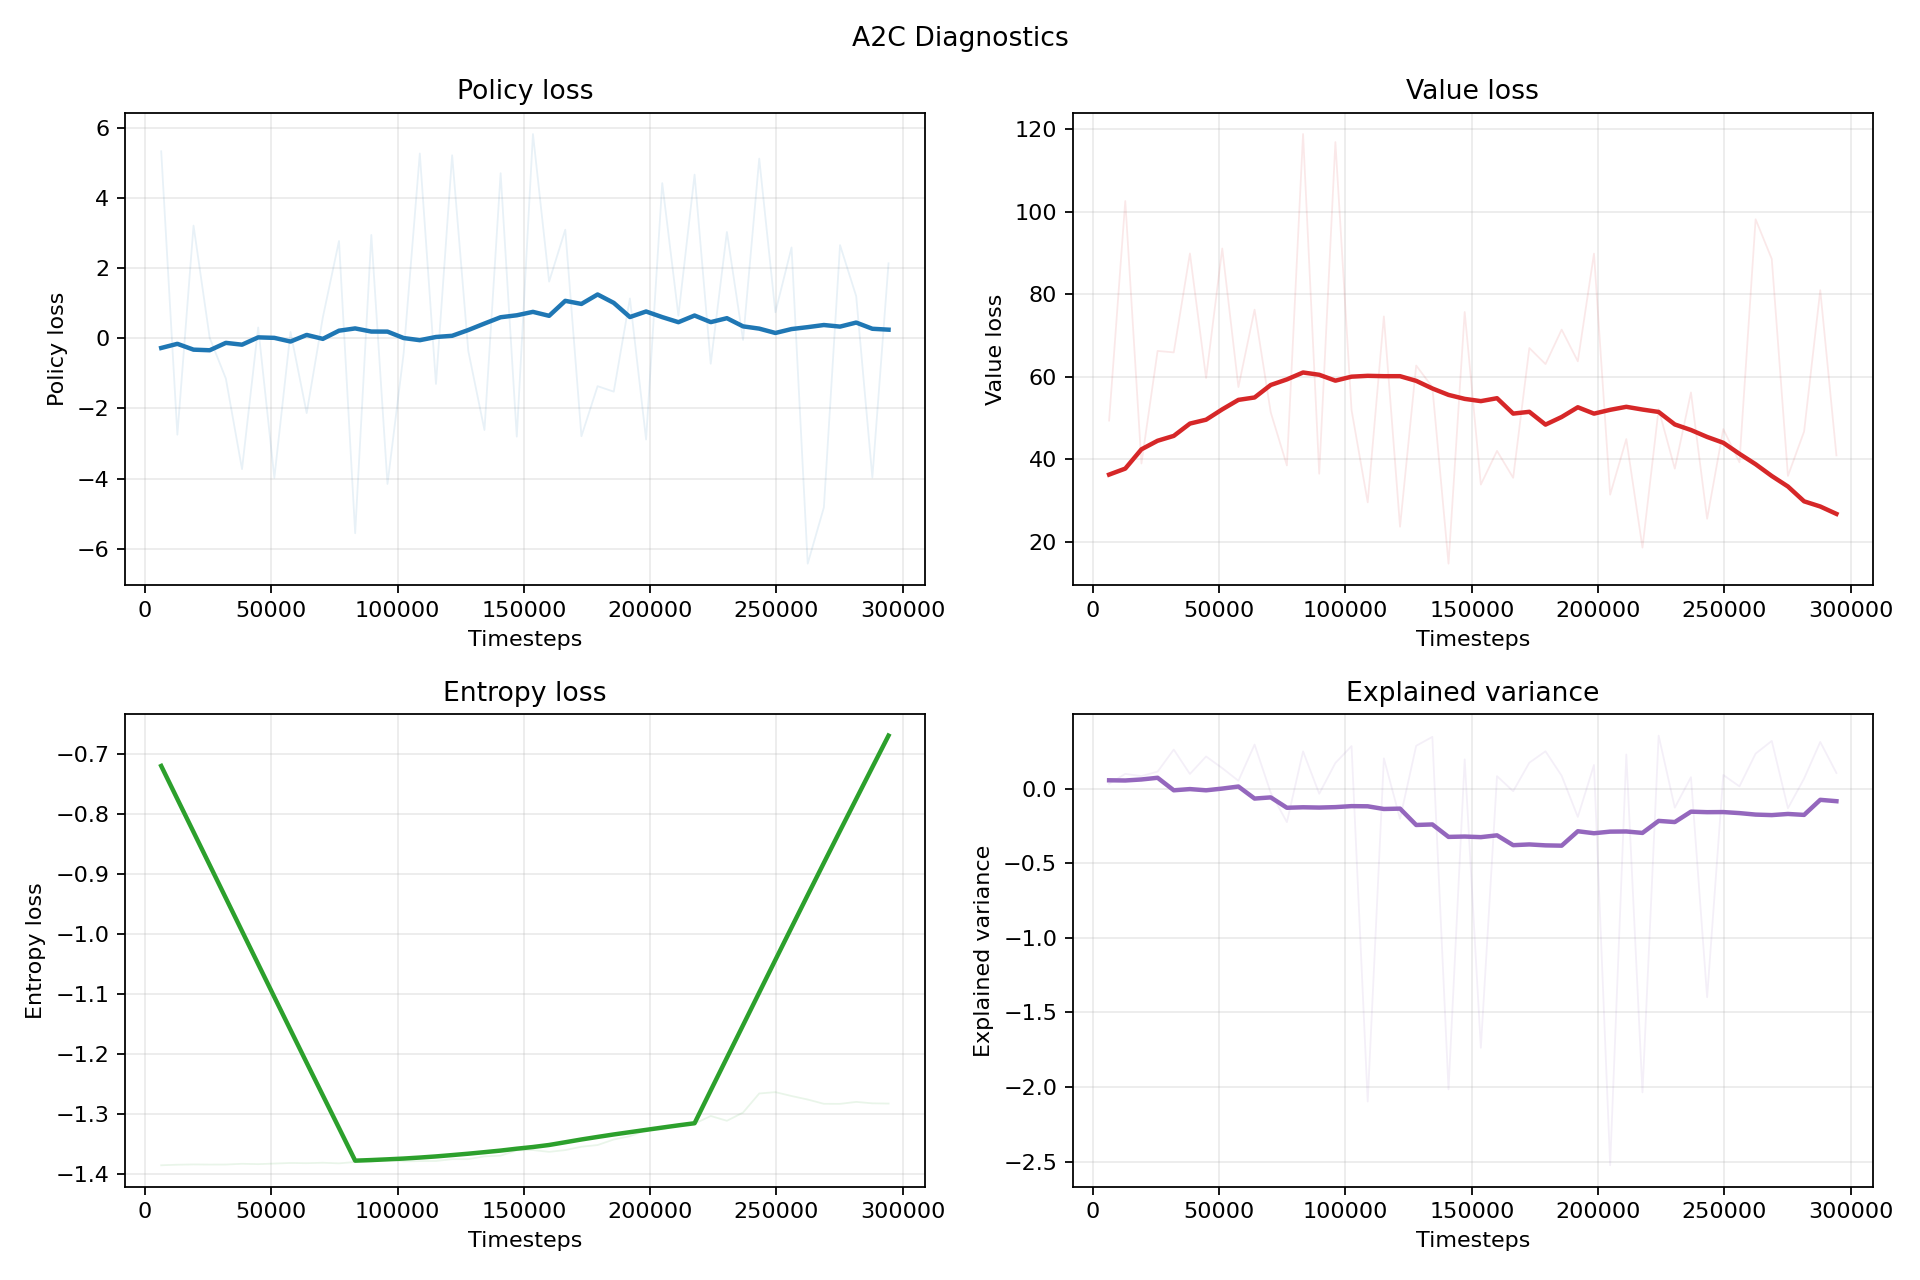
\includegraphics[width=0.92\textwidth]{graphics/chapter-6/train_A2C/a2c_diagnostics.png}
    \captionsetup{hypcap=false}
    \captionof{figure}{Biểu đồ chẩn đoán tổng hợp của A2C}
    \label{fig:a2c-diagnostics-summary}
\end{minipage}

\noindent Toàn bộ các thông số chẩn đoán huấn luyện của A2C được tổng hợp trực quan trong Hình \ref{fig:a2c-diagnostics-summary}. Sự nhất quán của cả bốn đồ thị thành phần khẳng định tiến trình học của A2C diễn ra ổn định và an toàn.

\begin{minipage}{\textwidth}
    \centering
    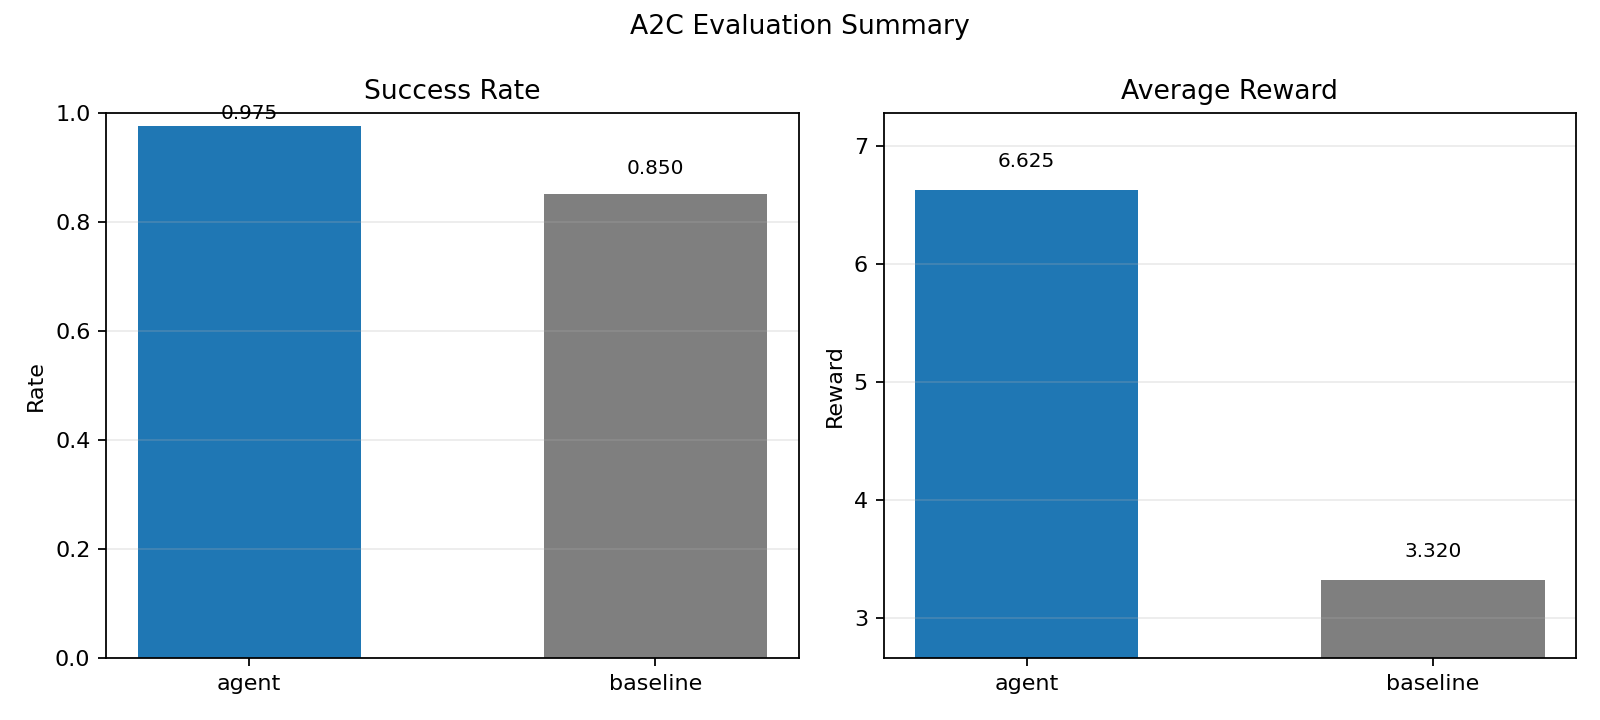
\includegraphics[width=0.92\textwidth]{graphics/chapter-6/train_A2C/evaluation_summary.png}
    \captionsetup{hypcap=false}
    \captionof{figure}{So sánh kết quả đánh giá A2C với baseline}
    \label{fig:a2c-evaluation-summary}
\end{minipage}

\noindent Kết quả đánh giá trong Hình \ref{fig:a2c-evaluation-summary} so sánh hiệu năng của tác nhân A2C sau huấn luyện với baseline ngẫu nhiên. Kết quả cho thấy tác nhân A2C đạt tỷ lệ phục hồi thành công vượt trội lên tới 0.975 (so với 0.850 của baseline). Đồng thời, phần thưởng trung bình đạt 6.625, cao gấp đôi so với mức 3.320 của baseline. Sự cải thiện vượt bậc này chứng minh tính hiệu quả của chính sách Actor-Critic trong việc tự phục hồi hệ thống khi xảy ra sự cố pod.


\subsection{PPO}

Đối với PPO, run huấn luyện được theo dõi trong khoảng 400\,000 bước thời gian. Trọng tâm của phần này là quan sát mức độ hội tụ của chính sách, độ ổn định của các đại lượng tối ưu hóa và kết quả đánh giá sau huấn luyện trên kịch bản \textit{pod failure}.

\begin{minipage}{\textwidth}
    \centering
    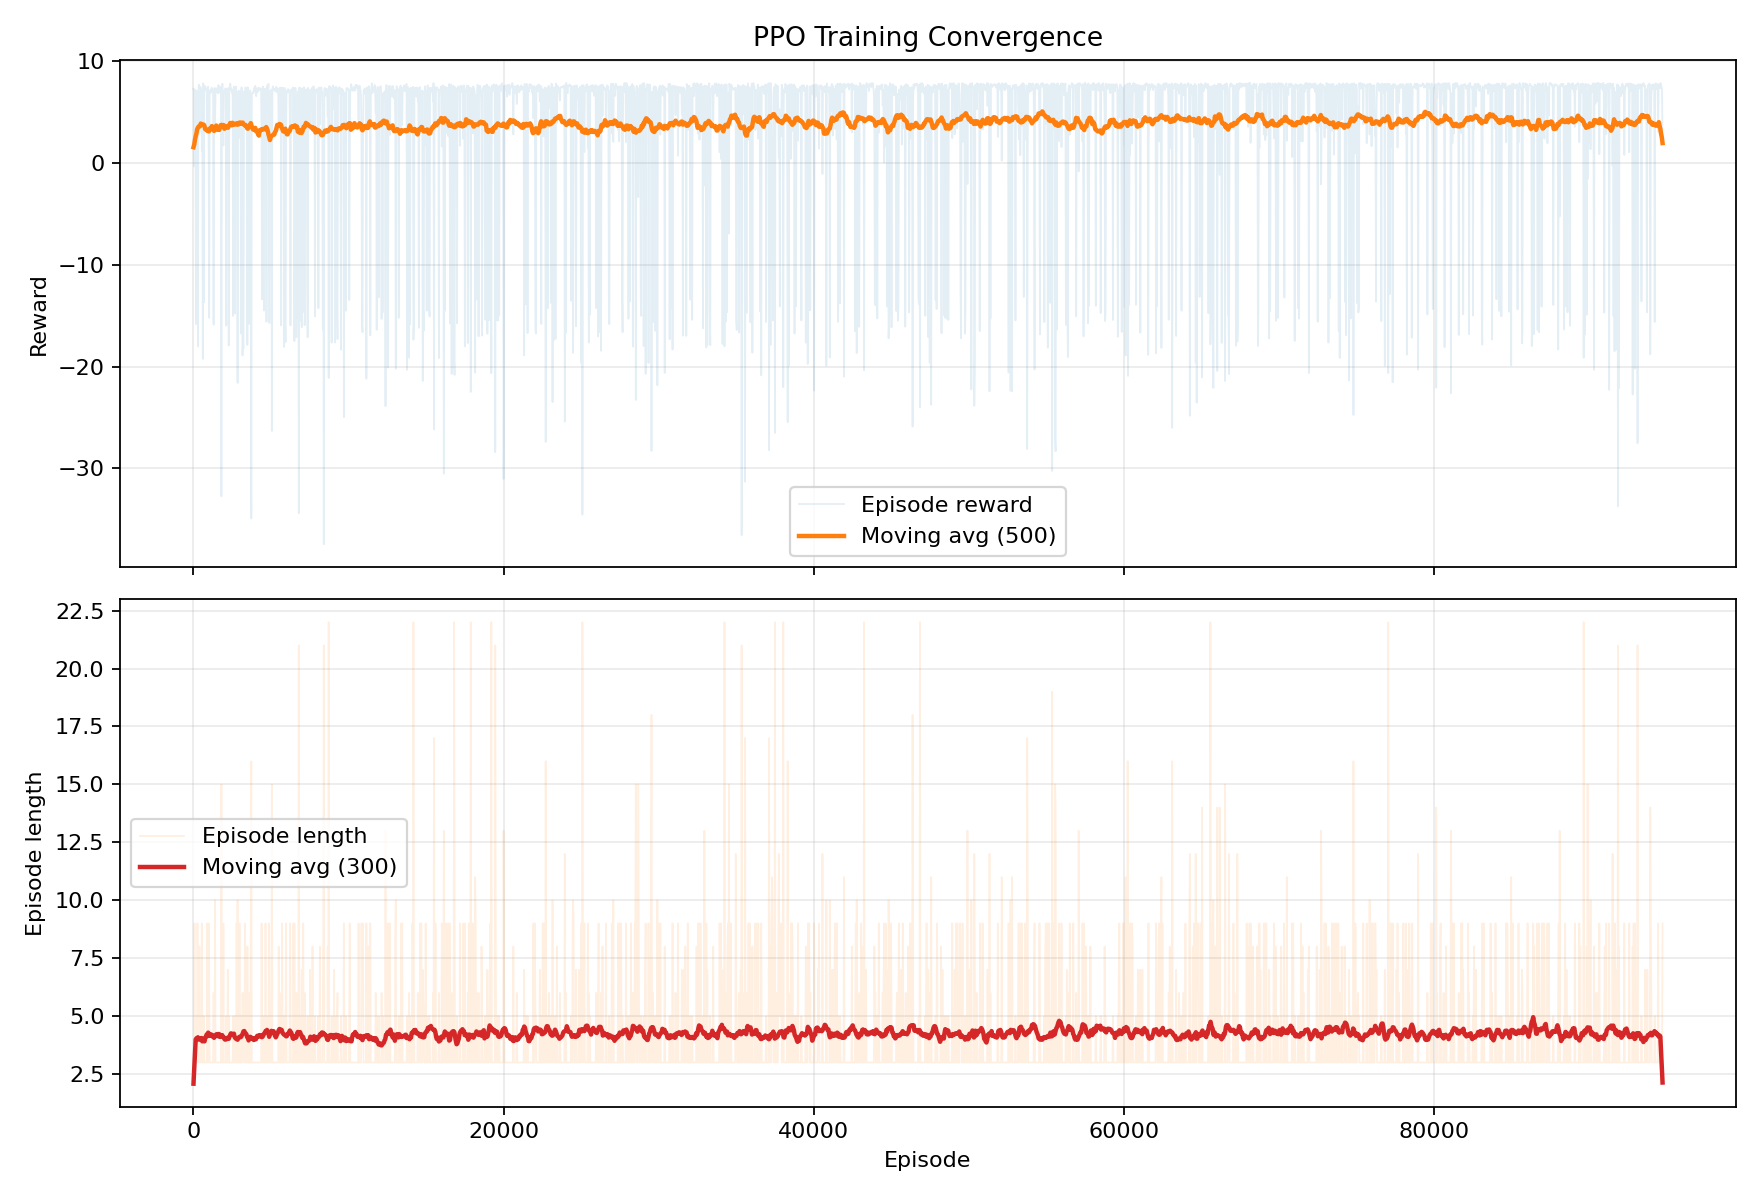
\includegraphics[width=0.95\textwidth]{graphics/chapter-6/train_PPO/training_curve.png}
    \captionsetup{hypcap=false}
    \captionof{figure}{Biểu đồ hội tụ theo phần thưởng và độ dài episode của PPO}
    \label{fig:ppo-training-convergence}
\end{minipage}

\noindent Hình \ref{fig:ppo-training-convergence} cho thấy phần thưởng theo episode có độ dao động lớn ở mức tức thời, phản ánh đúng bản chất nhiễu của môi trường replay từ dữ liệu thật. Tuy nhiên, đường trung bình trượt của phần thưởng duy trì xu hướng dương và tăng dần từ khoảng 3 lên trên 4, cho thấy chính sách PPO học được hành vi phục hồi ngày càng hiệu quả hơn. Ở đồ thị độ dài episode, giá trị trung bình ổn định quanh 4--5 bước, nghĩa là tác nhân thường đưa hệ thống về trạng thái phục hồi trong số bước tương đối ngắn.

\begin{minipage}{\textwidth}
    \centering
    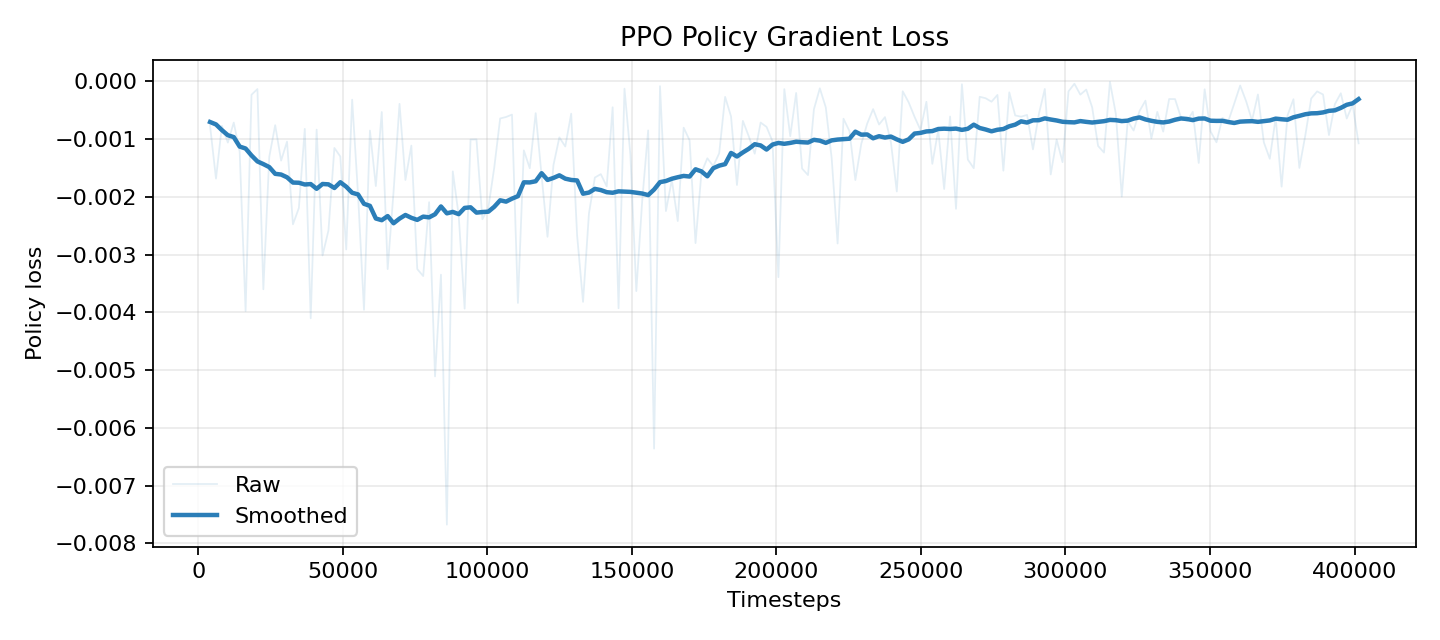
\includegraphics[width=0.9\textwidth]{graphics/chapter-6/train_PPO/policy_loss_curve.png}
    \captionsetup{hypcap=false}
    \captionof{figure}{Biến thiên \textit{policy loss} trong quá trình huấn luyện PPO}
    \label{fig:ppo-policy-loss}
\end{minipage}

\noindent Với Hình \ref{fig:ppo-policy-loss}, \textit{policy loss} ban đầu giảm xuống mức âm lớn hơn về độ lớn, sau đó tăng dần trở lại gần 0. Diễn biến này cho thấy ở giai đoạn đầu, chính sách thay đổi mạnh để nhanh chóng thích nghi với dữ liệu huấn luyện; về sau, độ lớn cập nhật giảm đi, phản ánh việc chính sách đã ổn định hơn và chỉ còn tinh chỉnh cục bộ.

\begin{minipage}{\textwidth}
    \centering
    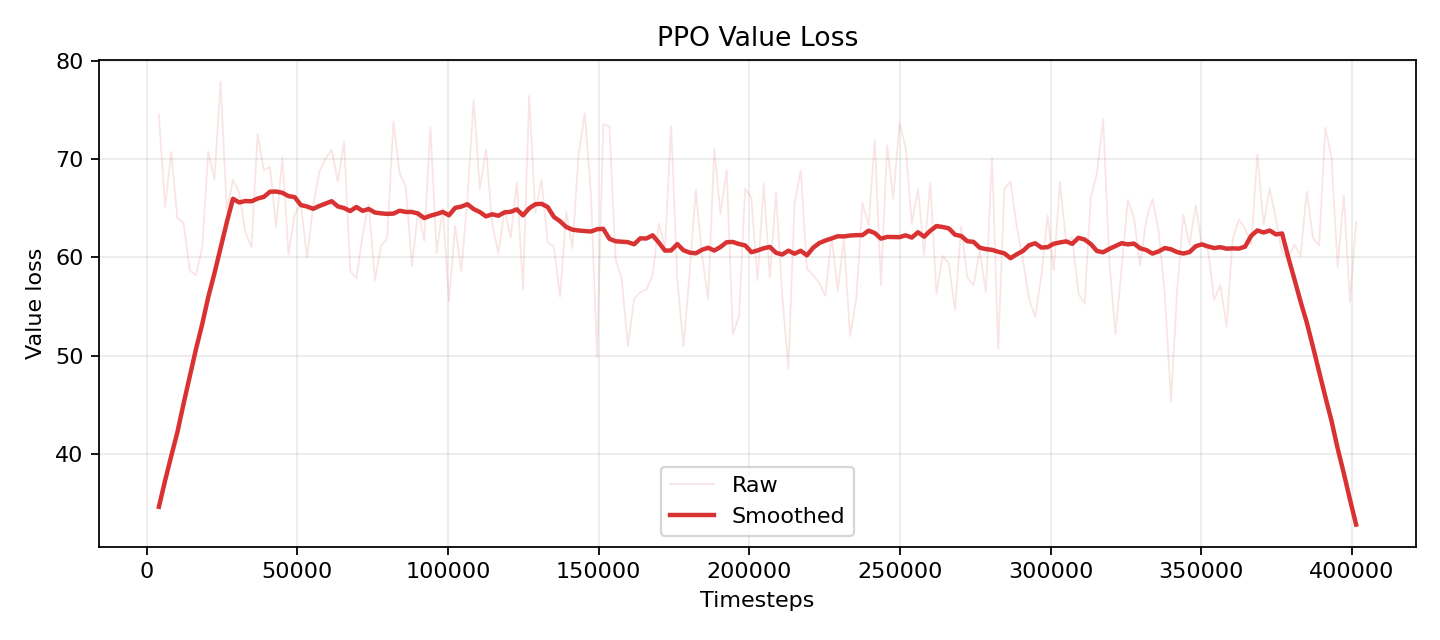
\includegraphics[width=0.9\textwidth]{graphics/chapter-6/train_PPO/value_loss_curve.png}
    \captionsetup{hypcap=false}
    \captionof{figure}{Biến thiên \textit{value loss} của PPO}
    \label{fig:ppo-value-loss}
\end{minipage}

\noindent Hình \ref{fig:ppo-value-loss} cho thấy \textit{value loss} dao động chủ yếu trong vùng 60--66 sau giai đoạn khởi đầu. Mặc dù vẫn còn nhiễu theo từng lần cập nhật, đường làm mượt không có xu hướng bùng nổ, qua đó cho thấy mạng giá trị giữ được sự ổn định trong suốt quá trình học. Phần giảm mạnh ở cuối đồ thị chủ yếu mang tính biên của đường làm mượt, vì vậy không nên diễn giải như một bước nhảy chất lượng đột ngột.

\begin{minipage}{\textwidth}
    \centering
    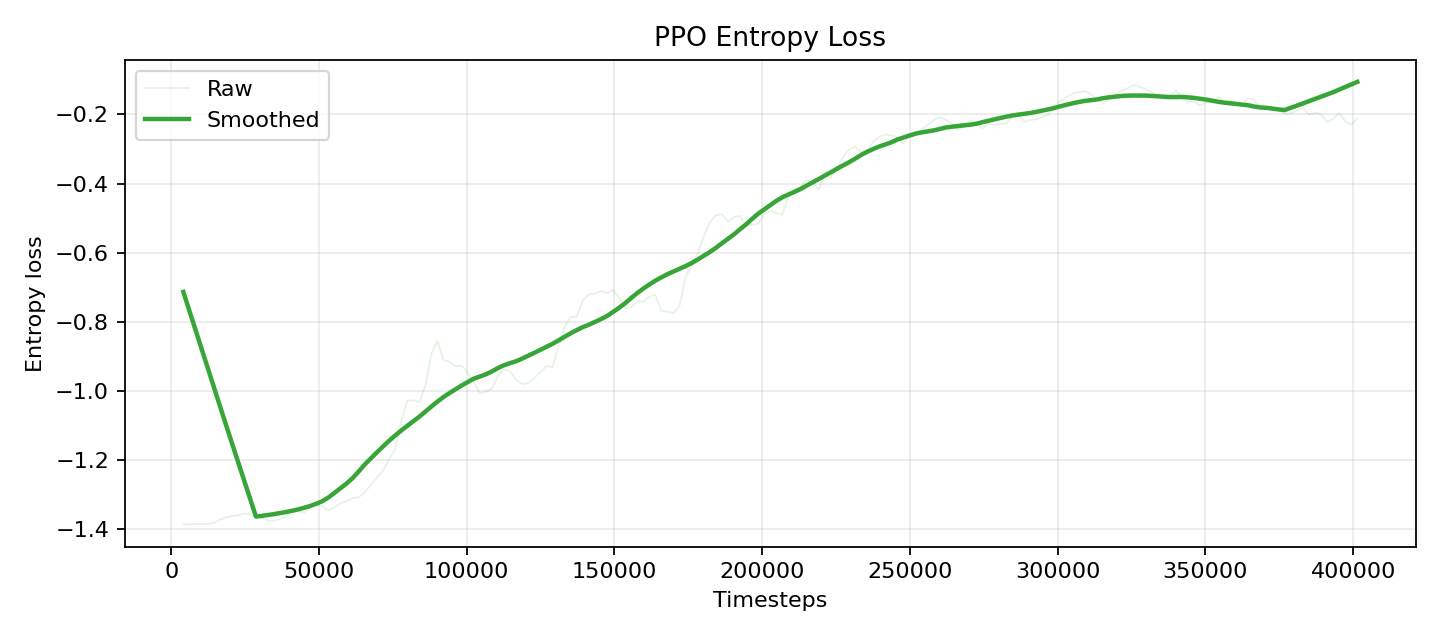
\includegraphics[width=0.9\textwidth]{graphics/chapter-6/train_PPO/entropy_curve.png}
    \captionsetup{hypcap=false}
    \captionof{figure}{Biến thiên \textit{entropy loss} của PPO}
    \label{fig:ppo-entropy-loss}
\end{minipage}

\noindent Ở Hình \ref{fig:ppo-entropy-loss}, \textit{entropy loss} dịch dần từ vùng âm lớn về gần 0. Điều này phản ánh entropy của chính sách giảm theo thời gian, tức là tác nhân bớt ngẫu nhiên hơn và ngày càng tập trung vào một tập hành động phục hồi nhất quán. Đây là tín hiệu tích cực, vì nó cho thấy PPO không chỉ học được mà còn dần củng cố một chính sách có tính quyết đoán hơn.

\begin{minipage}{\textwidth}
    \centering
    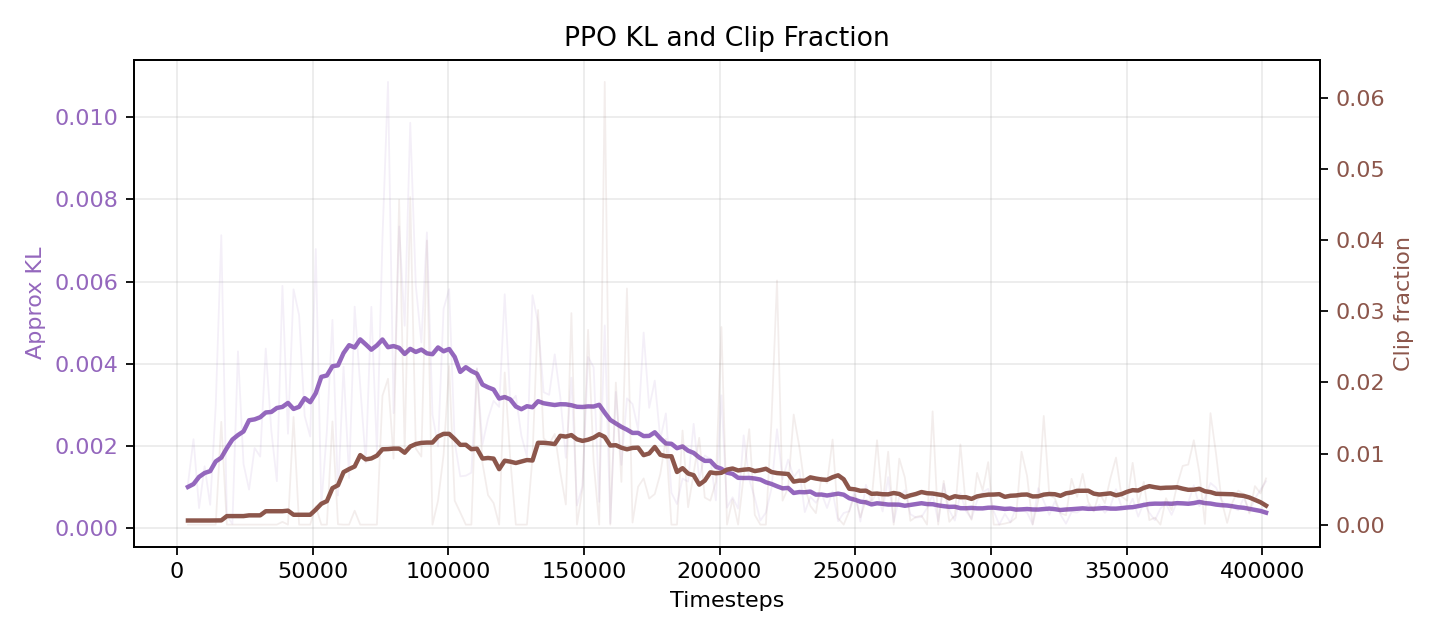
\includegraphics[width=0.92\textwidth]{graphics/chapter-6/train_PPO/kl_clip_curve.png}
    \captionsetup{hypcap=false}
    \captionof{figure}{Độ lệch KL xấp xỉ và \textit{clip fraction} trong PPO}
    \label{fig:ppo-kl-clip}
\end{minipage}

\noindent Hình \ref{fig:ppo-kl-clip} cho thấy \textit{approx KL} tăng dần ở giai đoạn đầu và đạt đỉnh khoảng 0.004--0.005 trước khi giảm về mức rất thấp ở cuối quá trình. Đồng thời, \textit{clip fraction} chỉ dao động quanh vùng nhỏ và cũng giảm dần sau nửa sau của quá trình học. Hai tín hiệu này cho thấy các bước cập nhật chính sách được kiểm soát tốt, không vượt quá ngưỡng thay đổi lớn và phù hợp với đặc trưng tối ưu hóa ổn định của PPO.

\begin{minipage}{\textwidth}
    \centering
    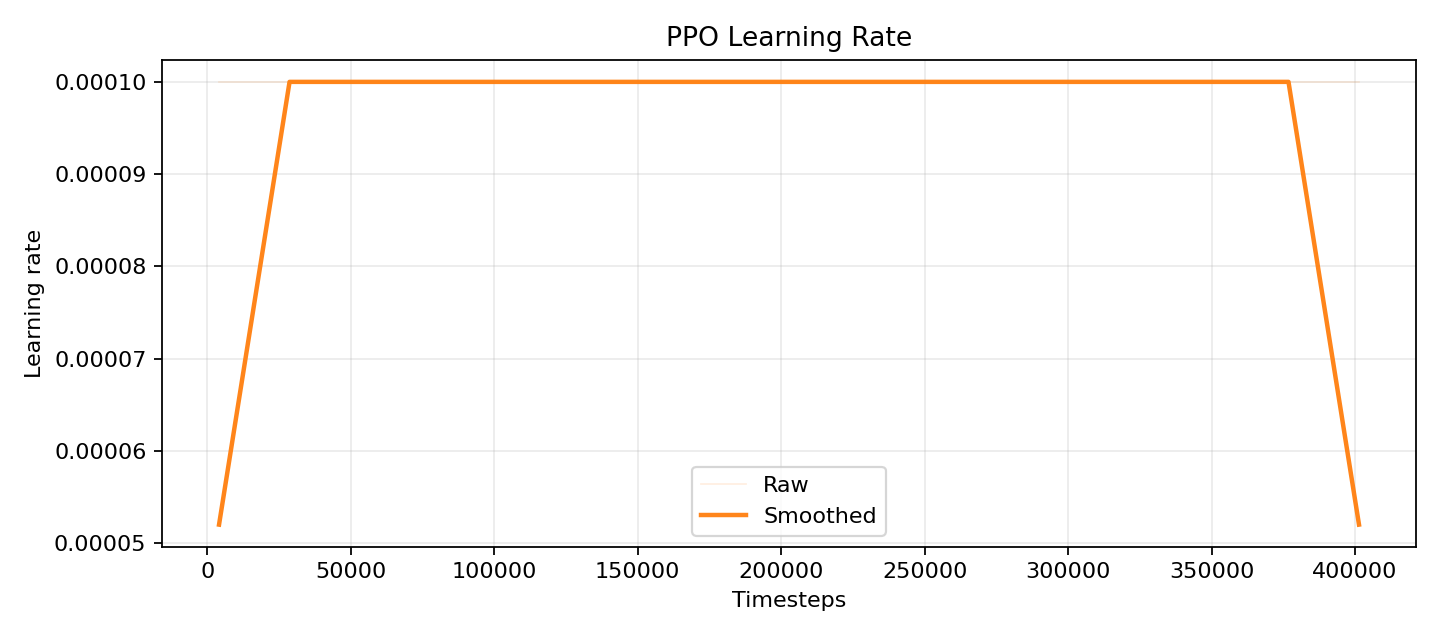
\includegraphics[width=0.9\textwidth]{graphics/chapter-6/train_PPO/learning_rate_curve.png}
    \captionsetup{hypcap=false}
    \captionof{figure}{Biến thiên tốc độ học trong quá trình huấn luyện PPO}
    \label{fig:ppo-learning-rate}
\end{minipage}

\noindent Từ Hình \ref{fig:ppo-learning-rate}, có thể thấy tốc độ học được duy trì gần như cố định quanh mức $10^{-4}$ trong phần lớn thời gian huấn luyện. Việc giữ \textit{learning rate} ổn định giúp PPO tránh được dao động tối ưu hóa quá mạnh, đồng thời tạo điều kiện để các chỉ số \textit{policy loss}, \textit{value loss} và \textit{approx KL} hội tụ theo hướng mượt hơn.

\begin{minipage}{\textwidth}
    \centering
    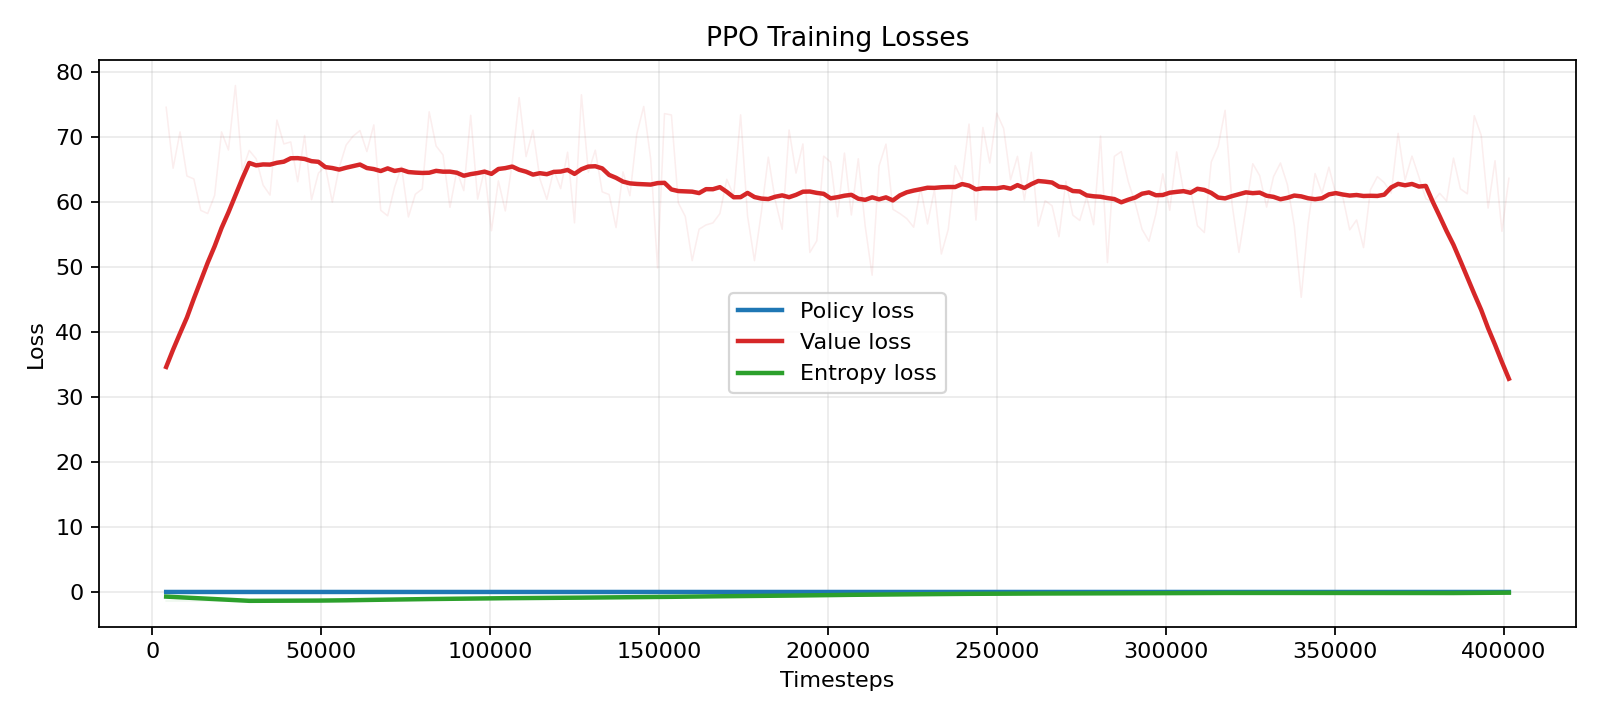
\includegraphics[width=0.92\textwidth]{graphics/chapter-6/train_PPO/loss_curve.png}
    \captionsetup{hypcap=false}
    \captionof{figure}{Biểu đồ tổng hợp các hàm mất mát chính của PPO}
    \label{fig:ppo-loss-summary}
\end{minipage}

\noindent Hình \ref{fig:ppo-loss-summary} tổng hợp đồng thời \textit{policy loss}, \textit{value loss} và \textit{entropy loss}. Có thể thấy \textit{value loss} chiếm thang đo lớn nhất, trong khi hai thành phần còn lại dao động nhỏ hơn nhiều. Dù khác thang đo, ba đại lượng đều giữ xu hướng ổn định theo thời gian và không xuất hiện hiện tượng phân kỳ, cho thấy quá trình học của actor và critic vẫn được duy trì cân bằng.

\begin{minipage}{\textwidth}
    \centering
    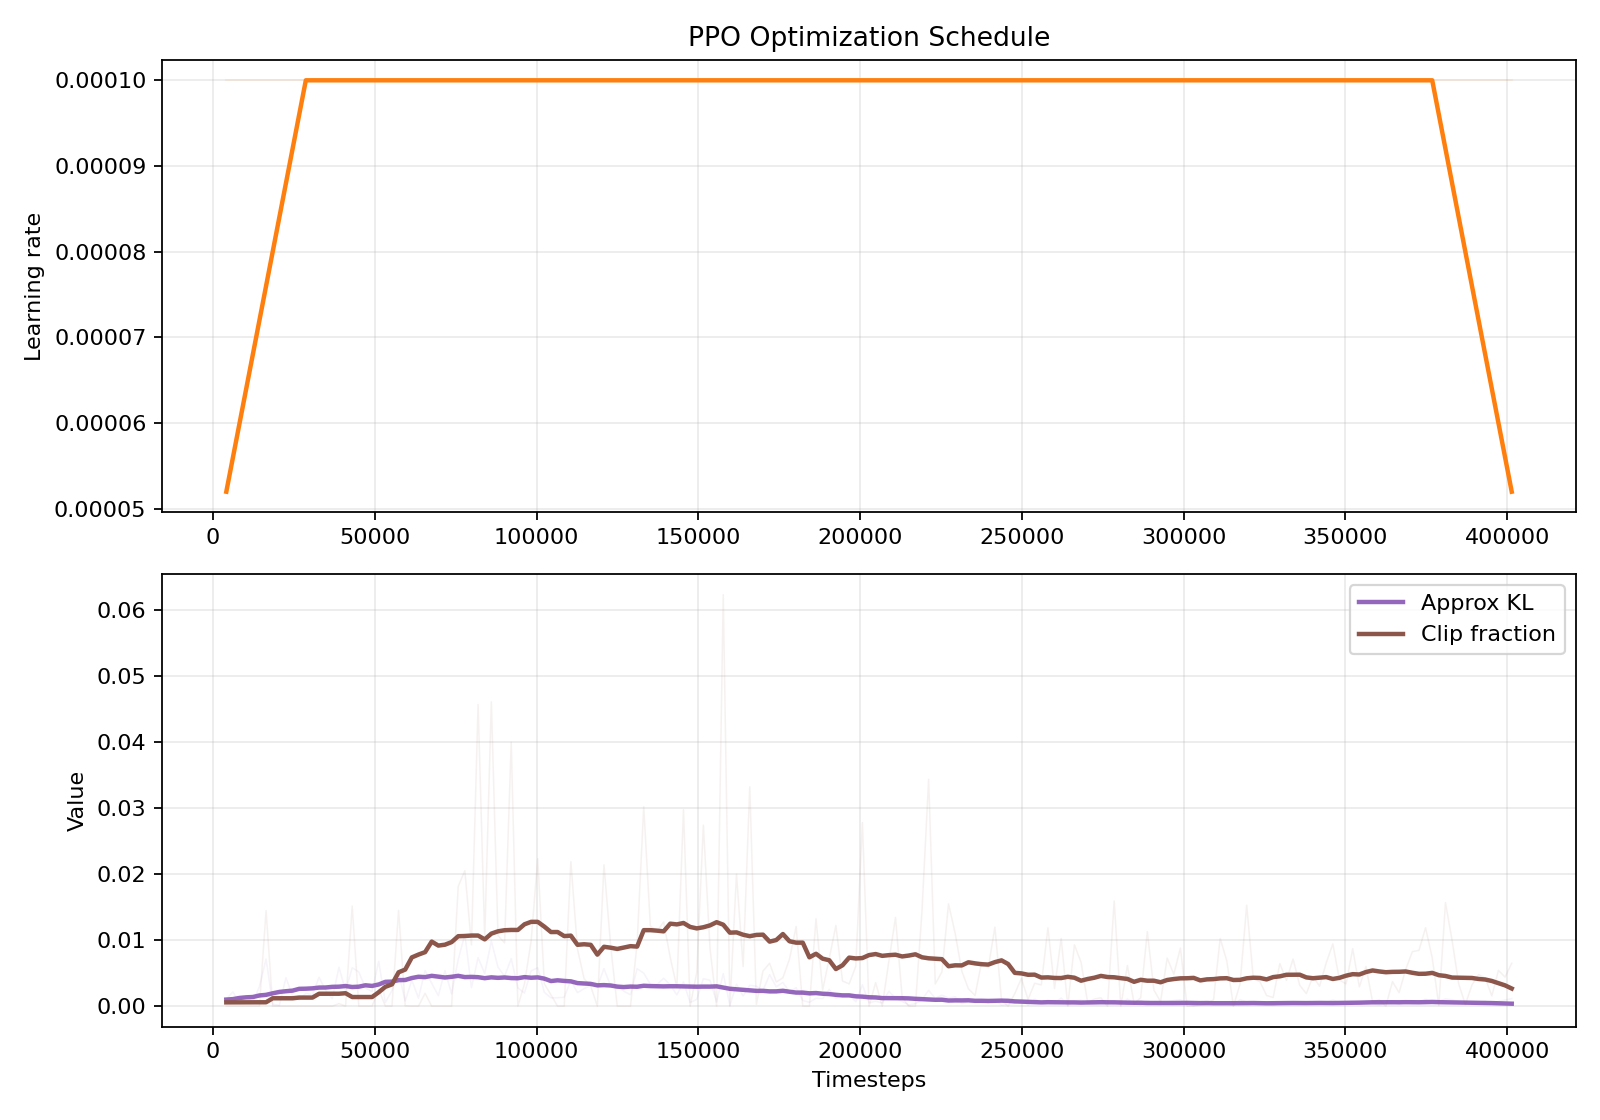
\includegraphics[width=0.92\textwidth]{graphics/chapter-6/train_PPO/optimization_curve.png}
    \captionsetup{hypcap=false}
    \captionof{figure}{Biểu đồ tổng hợp lịch tối ưu hóa và mức độ cập nhật chính sách của PPO}
    \label{fig:ppo-optimization-summary}
\end{minipage}

\noindent Hình \ref{fig:ppo-optimization-summary} cho thấy lại mối quan hệ giữa lịch tốc độ học, \textit{approx KL} và \textit{clip fraction} trong cùng một khung nhìn. Kết quả nhất quán với các đồ thị trước: tốc độ học ổn định, độ lệch KL được giữ nhỏ, và tỷ lệ bị clip không tăng đột biến. Điều này củng cố nhận định rằng PPO cập nhật chính sách theo hướng an toàn, phù hợp với bài toán yêu cầu hạn chế can thiệp quá mức lên hệ thống thật.

\begin{minipage}{\textwidth}
    \centering
    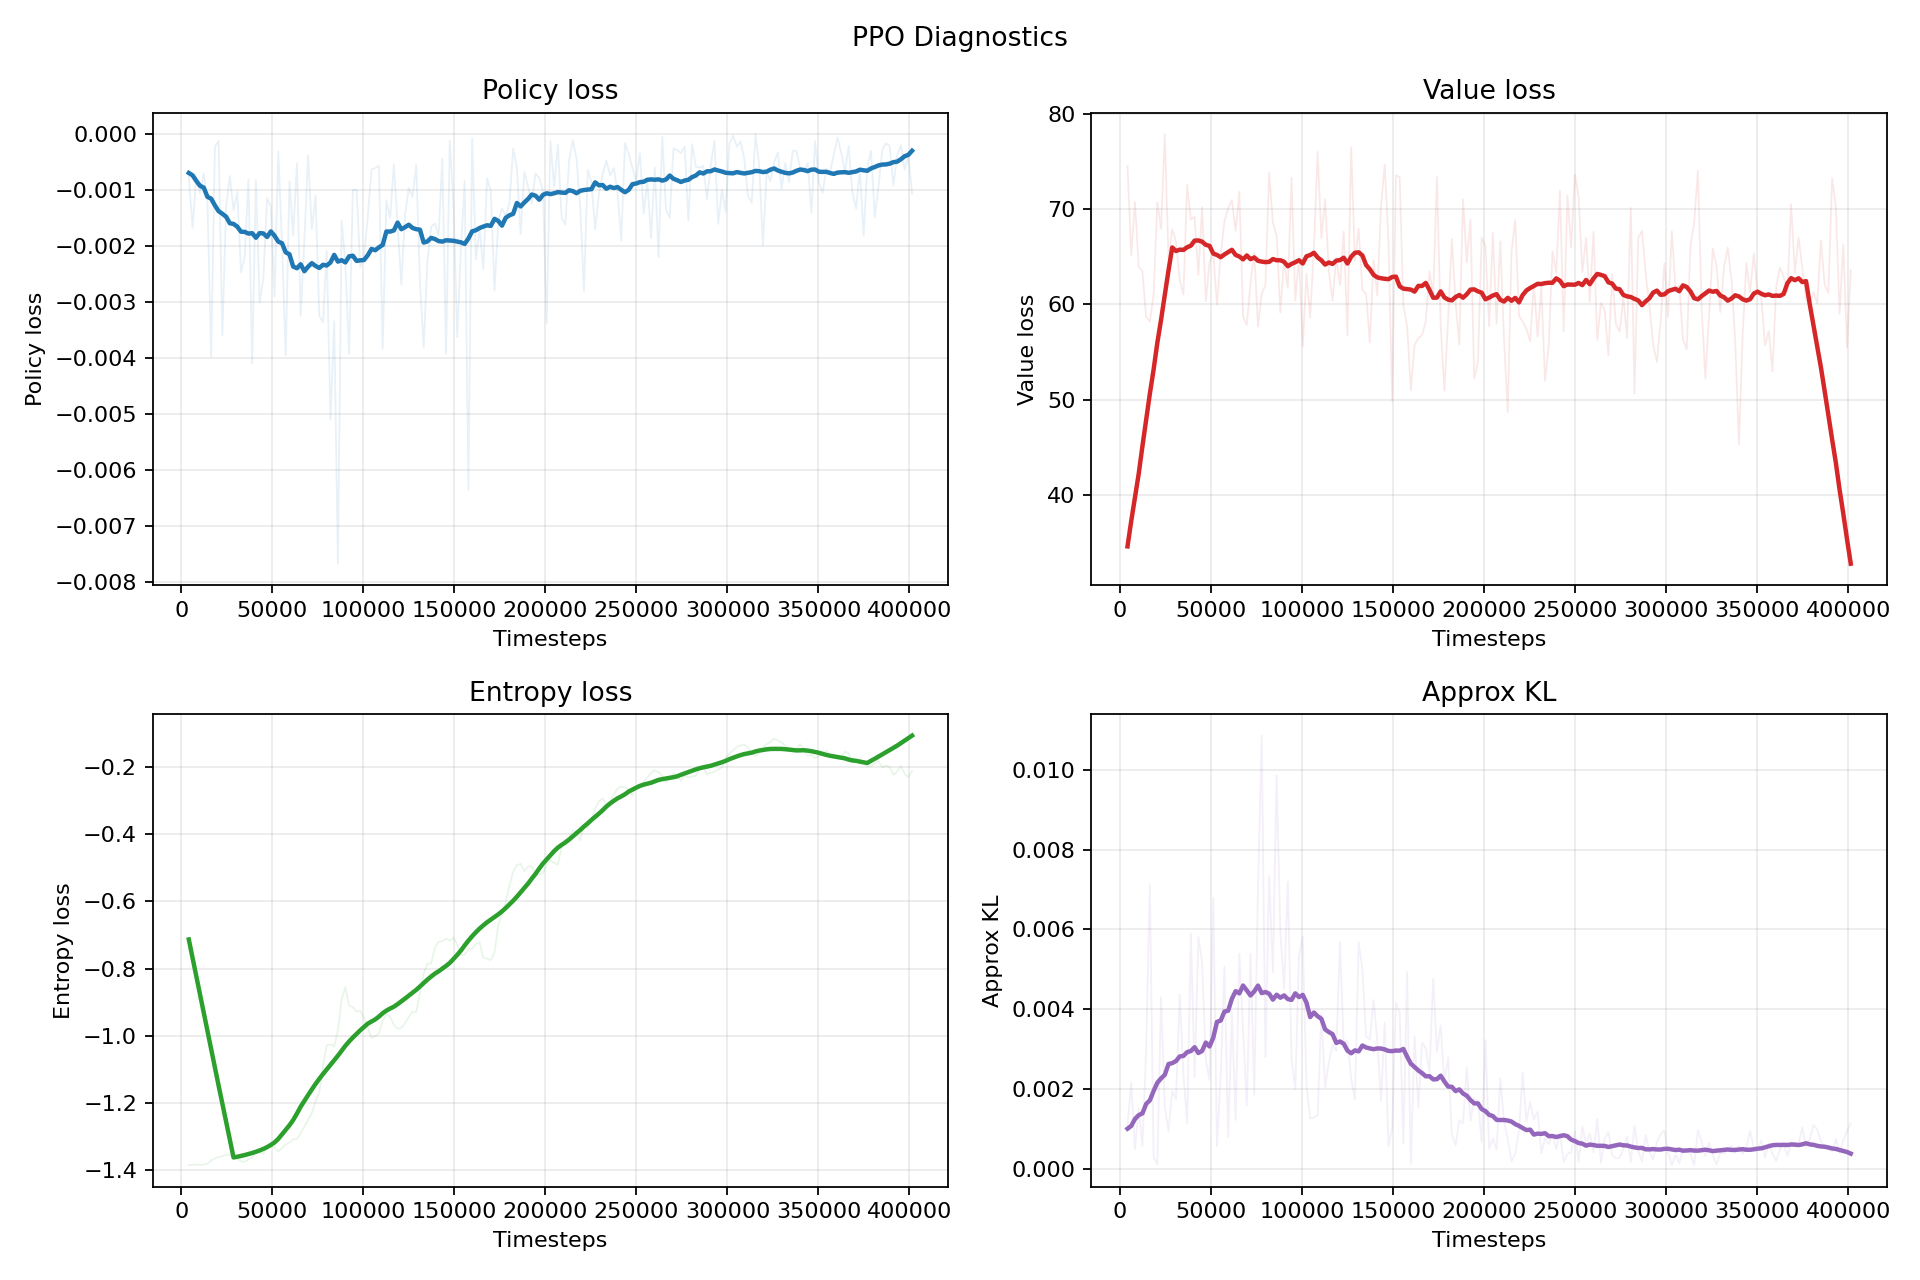
\includegraphics[width=0.92\textwidth]{graphics/chapter-6/train_PPO/ppo_diagnostics.png}
    \captionsetup{hypcap=false}
    \captionof{figure}{Biểu đồ chẩn đoán tổng hợp của PPO}
    \label{fig:ppo-diagnostics-summary}
\end{minipage}

\noindent Hình \ref{fig:ppo-diagnostics-summary} đóng vai trò đối chiếu nhanh toàn bộ các tín hiệu chẩn đoán quan trọng của PPO trong một trang duy nhất. Bốn đồ thị thành phần cùng chỉ ra một kết luận nhất quán: chính sách được cải thiện mạnh ở nửa đầu quá trình học, sau đó chuyển sang pha tinh chỉnh ổn định hơn ở nửa sau.

\begin{minipage}{\textwidth}
    \centering
    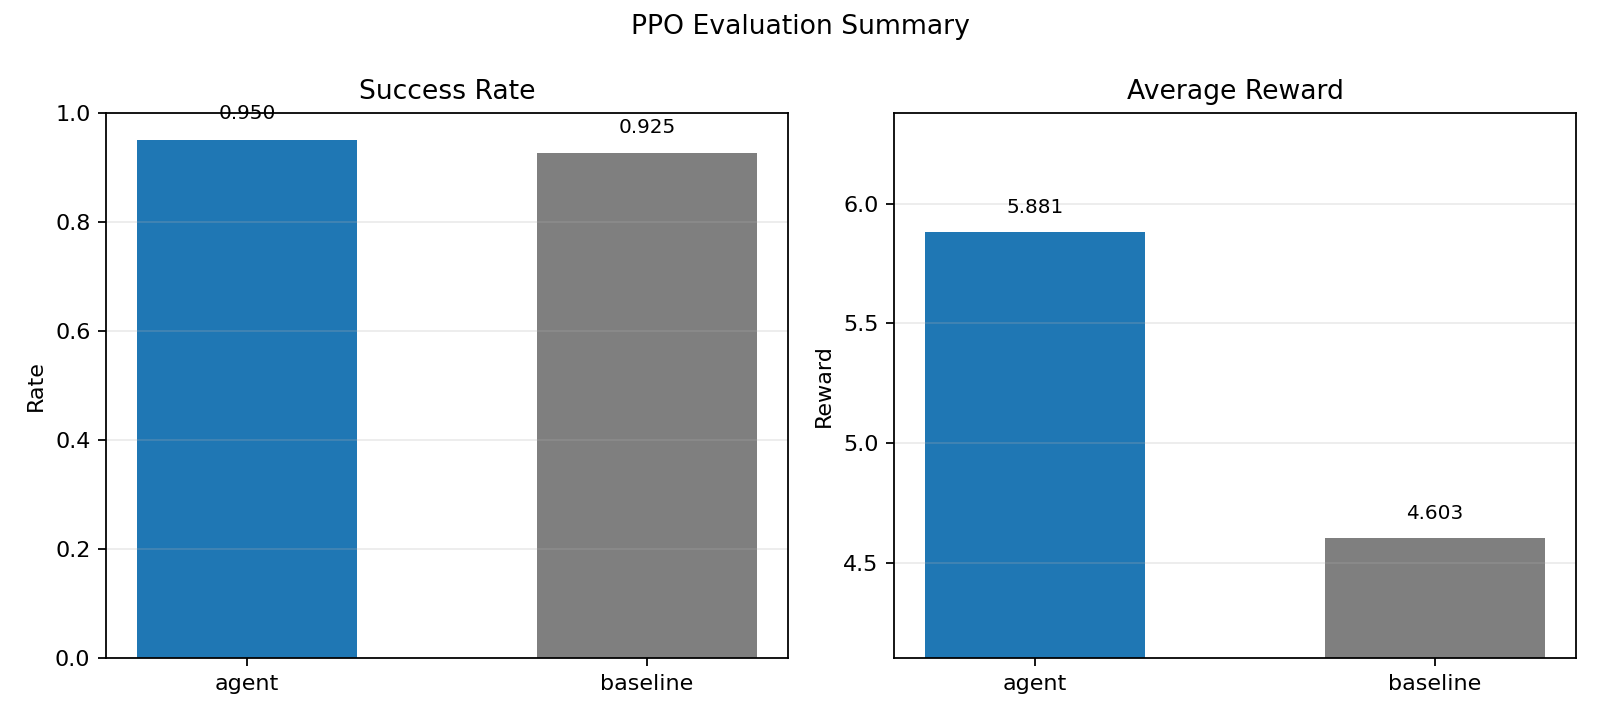
\includegraphics[width=0.92\textwidth]{graphics/chapter-6/train_PPO/evaluation_summary.png}
    \captionsetup{hypcap=false}
    \captionof{figure}{So sánh kết quả đánh giá PPO với baseline}
    \label{fig:ppo-evaluation-summary}
\end{minipage}

\noindent Tổng hợp các kết quả trên, PPO cho thấy ba đặc điểm tích cực trên kịch bản \textit{pod failure}: (i) đường phần thưởng hội tụ theo xu hướng tăng, (ii) các đại lượng tối ưu hóa như \textit{KL}, \textit{clip fraction} và các hàm mất mát được giữ trong miền ổn định, và (iii) kết quả đánh giá cuối cùng tốt hơn baseline cả về \textit{success rate} lẫn phần thưởng trung bình. Vì vậy, trong phạm vi thực nghiệm hiện tại, PPO là một ứng viên phù hợp cho bài toán tự phục hồi Kubernetes dựa trên học tăng cường.


\section{So sánh kết quả đánh giá offline giữa các thuật toán}

\noindent Sau khi hoàn thành giai đoạn huấn luyện riêng cho từng mô hình, nhóm tiến hành đánh giá offline trên cùng tập episode của kịch bản \textit{pod failure} để đối chiếu trực tiếp giữa DQN, A2C, PPO và baseline. Mục tiêu của phần này là xem xét không chỉ tỷ lệ phục hồi thành công, mà còn cả chất lượng hành vi can thiệp, độ dài chuỗi phục hồi và tác động của từng chính sách lên các chỉ số hệ thống quan trọng.

\begin{minipage}{\textwidth}
    \centering
    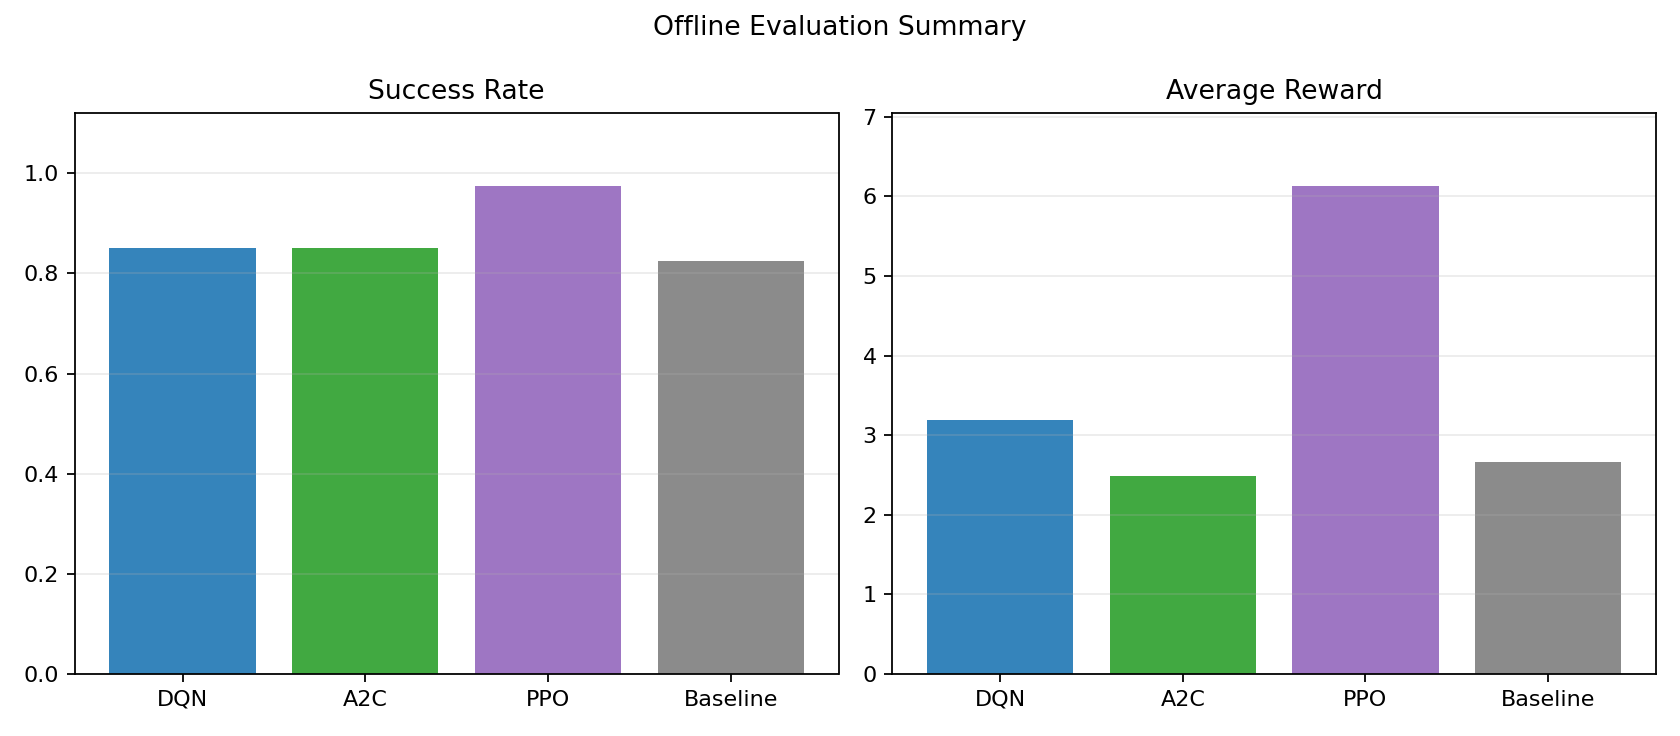
\includegraphics[width=0.92\textwidth]{graphics/chapter-6/compare/evaluation_summary.png}
    \captionsetup{hypcap=false}
    \captionof{figure}{Kết quả đánh giá offline tổng hợp của các thuật toán}
    \label{fig:compare-evaluation-summary}
\end{minipage}

\noindent Hình \ref{fig:compare-evaluation-summary} trình bày hai đại lượng tổng quát nhất của pha đánh giá offline là \textit{success rate} và \textit{average reward}. Có thể thấy PPO đạt kết quả nổi bật nhất với tỷ lệ thành công xấp xỉ 0.97 và phần thưởng trung bình trên 6.0. Trong khi đó, DQN và A2C cùng đạt mức \textit{success rate} khoảng 0.85, đều cao hơn baseline khoảng 0.82. Xét theo phần thưởng trung bình, DQN đạt khoảng 3.2, baseline khoảng 2.6 và A2C khoảng 2.5. Kết quả này cho thấy PPO không chỉ phục hồi thành công với tần suất cao hơn mà còn tạo ra chuỗi hành động có chất lượng tốt hơn theo đúng hàm thưởng đã thiết kế.

\begin{minipage}{\textwidth}
    \centering
    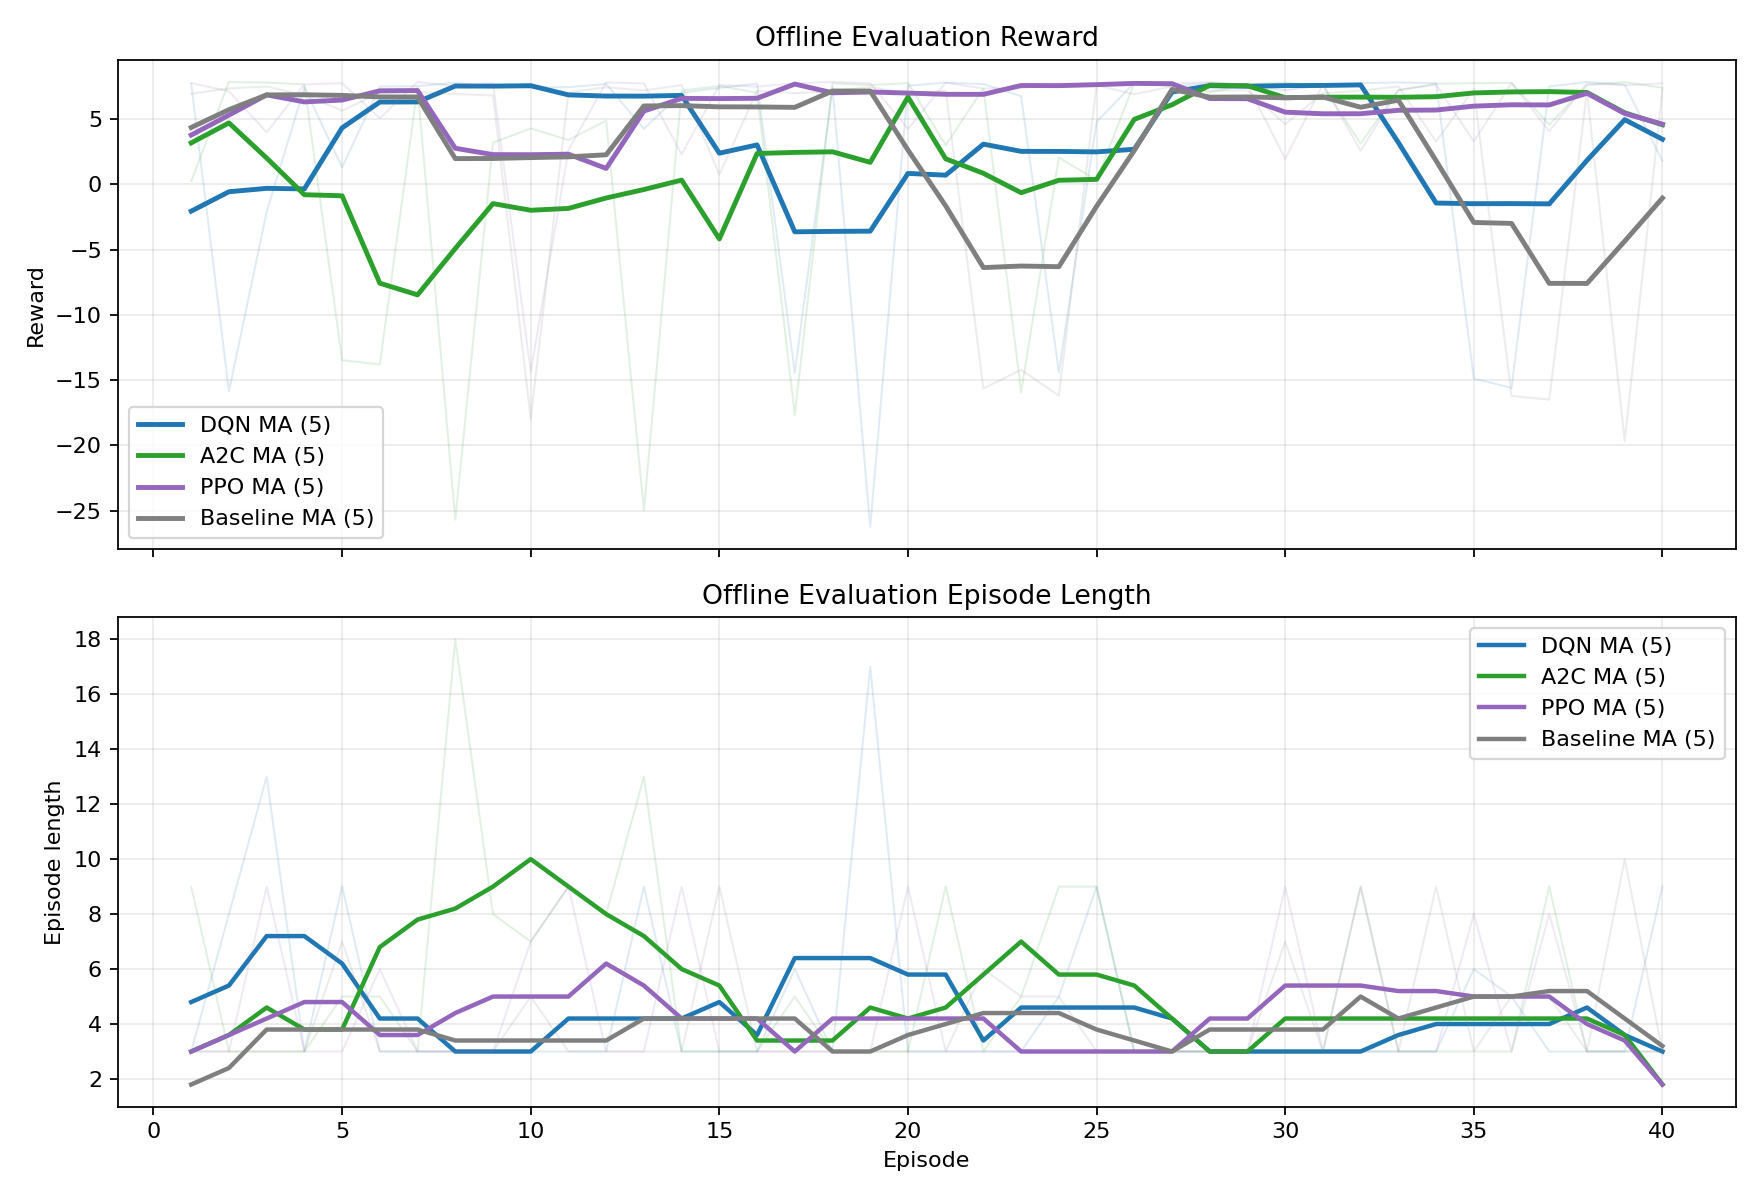
\includegraphics[width=0.95\textwidth]{graphics/chapter-6/compare/episode_curves.png}
    \captionsetup{hypcap=false}
    \captionof{figure}{Biến thiên phần thưởng và độ dài episode trong các tập đánh giá}
    \label{fig:compare-episode-curves}
\end{minipage}

\noindent Diễn biến chi tiết theo từng episode được thể hiện trong Hình \ref{fig:compare-episode-curves}. Đường trung bình trượt MA(5) của PPO duy trì ở vùng cao và ổn định nhất trong cả hai khía cạnh: phần thưởng thường nằm trong vùng dương cao, còn độ dài episode chủ yếu dao động quanh 3--5 bước. DQN cho kết quả trung bình khá hơn baseline nhưng vẫn xuất hiện một số đoạn giảm reward rõ rệt ở các episode khó. A2C có giai đoạn reward giảm sâu hơn DQN và PPO, đồng thời độ dài episode biến động mạnh hơn ở nửa đầu tập đánh giá. Nhìn chung, biểu đồ này củng cố nhận định rằng PPO có độ ổn định tốt nhất khi đối mặt với nhiều quỹ đạo lỗi khác nhau, trong khi DQN đứng ở vị trí trung gian và A2C nhạy hơn với các episode bất lợi.

\begin{minipage}{\textwidth}
    \centering
    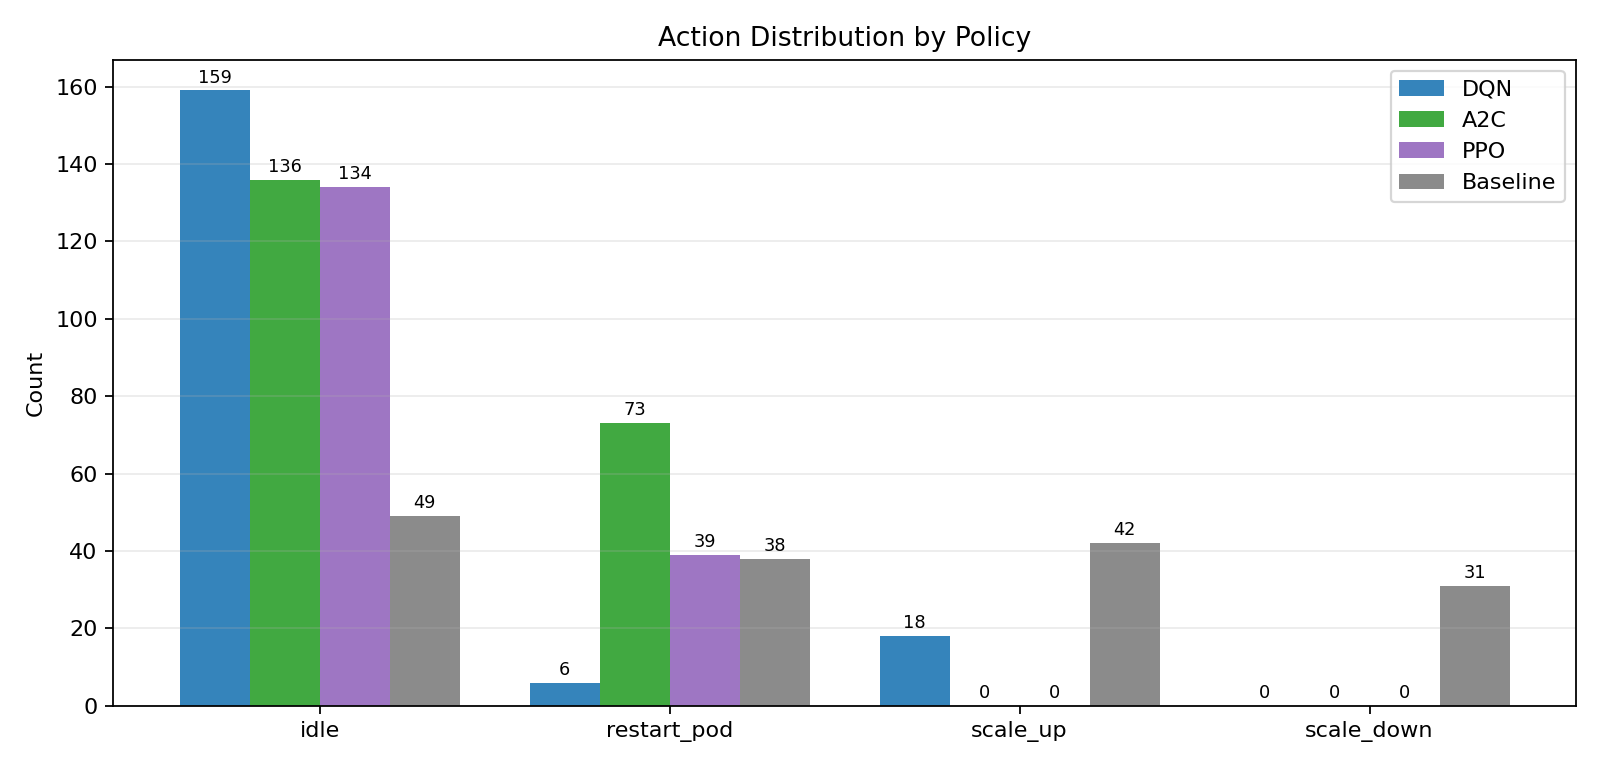
\includegraphics[width=0.92\textwidth]{graphics/chapter-6/compare/action_distribution.png}
    \captionsetup{hypcap=false}
    \captionof{figure}{Phân phối các hành động can thiệp của các thuật toán}
    \label{fig:compare-action-distribution}
\end{minipage}

\noindent Hình \ref{fig:compare-action-distribution} cho thấy sự khác biệt khá rõ trong cách ba tác nhân RL phân bổ hành động. Cả DQN, A2C và PPO đều ưu tiên mạnh hành động \texttt{idle}, với số lần lựa chọn lớn hơn nhiều so với baseline. Điều này phản ánh khả năng tránh can thiệp không cần thiết khi hệ thống đã ổn định. Ở nhóm hành động khôi phục trực tiếp, A2C sử dụng \texttt{restart\_pod} nhiều nhất (73 lần), PPO sử dụng ở mức vừa phải (39 lần), còn DQN chỉ dùng 6 lần nhưng lại thực hiện \texttt{scale\_up} 18 lần. Baseline phân bố hành động rải đều hơn, bao gồm cả \texttt{scale\_down}, cho thấy chính sách đối chứng thiếu xu hướng tập trung vào hành vi phục hồi đặc thù. Từ góc nhìn vận hành, PPO cho thấy cân bằng tốt giữa hai yêu cầu: hạn chế can thiệp thừa và vẫn giữ đủ khả năng phản ứng khi lỗi pod thực sự xảy ra.

\begin{minipage}{\textwidth}
    \centering
    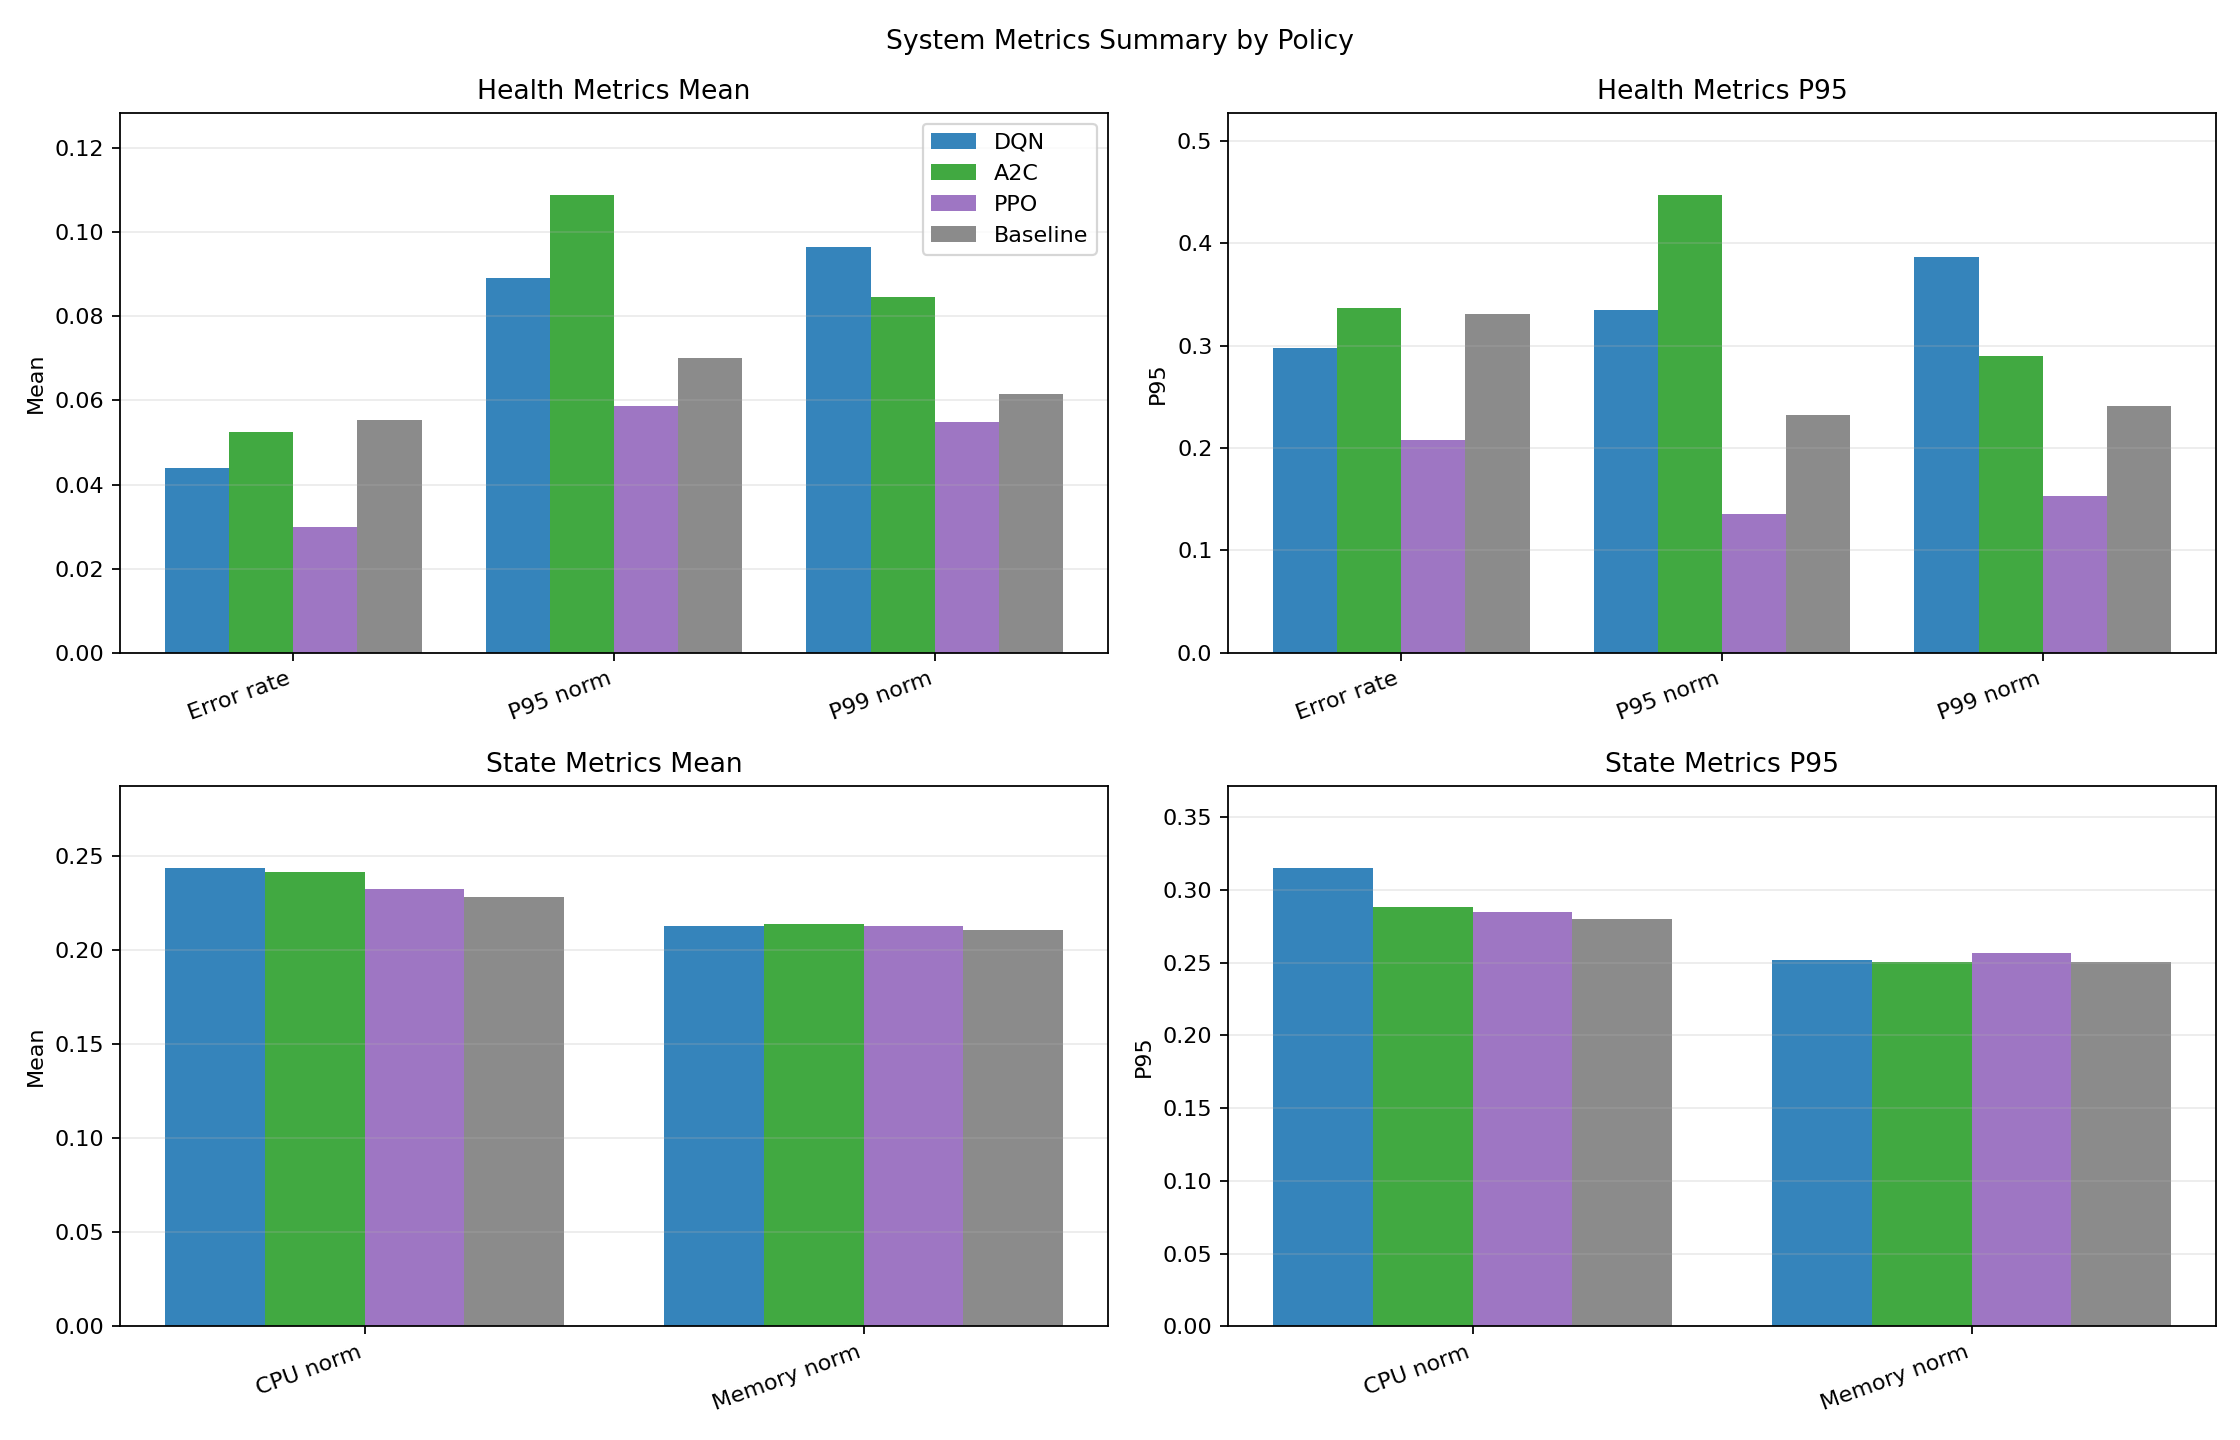
\includegraphics[width=0.95\textwidth]{graphics/chapter-6/compare/system_metrics_summary.png}
    \captionsetup{hypcap=false}
    \captionof{figure}{Tổng hợp các chỉ số hệ thống và trạng thái theo từng chính sách}
    \label{fig:compare-system-metrics}
\end{minipage}

\noindent Hình \ref{fig:compare-system-metrics} tổng hợp các chỉ số hệ thống chính dưới dạng giá trị trung bình và phân vị 95 cho bốn chính sách. Với nhóm chỉ số sức khỏe dịch vụ, PPO cho kết quả tốt nhất hoặc gần tốt nhất ở cả \textit{error rate}, \textit{p95\_norm} và \textit{p99\_norm}; đặc biệt, độ trễ ở các phân vị cao của PPO thấp hơn rõ rệt so với DQN và A2C. DQN có mức \textit{error rate} trung bình thấp hơn baseline nhưng phần đuôi độ trễ vẫn còn cao, còn A2C cho thấy \textit{p95\_norm} và \textit{p99\_norm} biến động lớn hơn. Ở nhóm chỉ số trạng thái như \textit{CPU norm} và \textit{Memory norm}, chênh lệch giữa các chính sách là không lớn, cho thấy khác biệt hiệu năng chủ yếu đến từ chất lượng ra quyết định phục hồi hơn là do một chính sách tiêu tốn tài nguyên vượt trội so với phần còn lại.

\noindent Tổng hợp bốn góc nhìn trên, có thể rút ra ba nhận xét chính. Thứ nhất, PPO là thuật toán cho kết quả tốt nhất về tổng thể khi đồng thời đạt \textit{success rate} cao nhất, phần thưởng trung bình cao nhất và các chỉ số sức khỏe dịch vụ thấp nhất. Thứ hai, DQN vẫn cho kết quả tốt hơn baseline ở cả khả năng phục hồi lẫn reward, nhưng hành vi can thiệp còn thận trọng quá mức ở \texttt{restart\_pod} và đôi khi lệch sang \texttt{scale\_up}. Thứ ba, A2C có khả năng phục hồi thành công ở mức khá nhưng độ ổn định giữa các episode chưa đồng đều bằng PPO. Vì vậy, trong phạm vi đánh giá offline của đồ án, PPO là mô hình phù hợp nhất để tiếp tục xem xét cho bước triển khai và điều khiển self-healing trên hệ thống Kubernetes.
